%% Preamble %%
%% A minimal LaTeX preamble
%% Some packates are needed to implement
%% Asciidoc features


\documentclass[11pt]{amsbook}
\usepackage{geometry}                % See geometry.pdf to learn the layout options. There are lots.
\geometry{letterpaper}               % ... or a4paper or a5paper or ...
%\geometry{landscape}                % Activate for for rotated page geometry

\documentclass[11pt]{amsart}
\usepackage{geometry}                % See geometry.pdf to learn the layout options. There are lots.
\geometry{letterpaper}               % ... or a4paper or a5paper or ...
%\geometry{landscape}                % Activate for for rotated page geometry
%\usepackage[parfill]{parskip}       % Activate to begin paragraphs with an empty line rather than an indent

\usepackage{tcolorbox}
\usepackage{lipsum}

\usepackage{epstopdf}
\usepackage{color}
% \usepackage[usenames, dvipsnames]{color}
% \usepackage{alltt}


\usepackage{amssymb}
% \usepackage{amsmath}
\usepackage{amsthm}
\usepackage[version=3]{mhchem}


% Needed to properly typeset
% standard unicode characters:
%
\RequirePackage{fix-cm}
\usepackage{fontspec}
\usepackage[Latin,Greek]{ucharclasses}
%
% NOTE: you must also use xelatex
% as the typesetting engine


% \usepackage{fontspec}
% \usepackage{polyglossia}
% \setmainlanguage{en}

\usepackage{hyperref}
\hypersetup{
    colorlinks=true,
    linkcolor=blue,
    filecolor=magenta,
    urlcolor=cyan,
}

\usepackage{graphicx}
\usepackage{wrapfig}
\graphicspath{ {images/} }
\DeclareGraphicsExtensions{.png, .jpg, jpeg, .pdf}

%% \DeclareGraphicsRule{.tif}{png}{.png}{`convert #1 `dirname #1`/`basename #1 .tif`.png}
%% Asciidoc TeX Macros %%


% \pagecolor{black}
%%%%%%%%%%%%


% Needed for Asciidoc

\newcommand{\admonition}[2]{\textbf{#1}: {#2}}
\newcommand{\rolered}[1]{ \textcolor{red}{#1} }
\newcommand{\roleblue}[1]{ \textcolor{blue}{#1} }

\newtheorem{theorem}{Theorem}
\newtheorem{proposition}{Proposition}
\newtheorem{corollary}{Corollary}
\newtheorem{lemma}{Lemma}
\newtheorem{definition}{Definition}
\newtheorem{conjecture}{Conjecture}
\newtheorem{problem}{Problem}
\newtheorem{exercise}{Exercise}
\newtheorem{example}{Example}
\newtheorem{note}{Note}
\newtheorem{joke}{Joke}
\newtheorem{objection}{Objection}





%%%%%%%%%%%%%%%%%%%%%%%%%%%%%%%%%%%%%%%%%%%%%%%%%%%%%%%

%  Extended quote environment with author

\renewenvironment{quotation}
{   \leftskip 4em \begin{em} }
{\end{em}\par }

\def\signed#1{{\leavevmode\unskip\nobreak\hfil\penalty50\hskip2em
  \hbox{}\nobreak\hfil\raise-3pt\hbox{(#1)}%
  \parfillskip=0pt \finalhyphendemerits=0 \endgraf}}


\newsavebox\mybox

\newenvironment{aquote}[1]
  {\savebox\mybox{#1}\begin{quotation}}
  {\signed{\usebox\mybox}\end{quotation}}

\newenvironment{tquote}[1]
  {  {\bf #1} \begin{quotation} \\ }
  { \end{quotation} }

%% BOXES: http://tex.stackexchange.com/questions/83930/what-are-the-different-kinds-of-boxes-in-latex
%% ENVIRONMENTS: https://www.sharelatex.com/learn/Environments

\newenvironment{asciidocbox}
  {\leftskip6em\rightskip6em\par}
  {\par}

\newenvironment{titledasciidocbox}[1]
  {\leftskip6em\rightskip6em\par{\bf #1}\vskip-0.6em\par}
  {\par}



%%%%%%%%%%%%%%%%%%%%%%%%%%%%%%%%%%%%%%%%%%%%%%%%%%%%%%%%

%% http://texblog.org/tag/rightskip/


\newenvironment{preamble}
  {}
  {}

%% http://tex.stackexchange.com/questions/99809/box-or-sidebar-for-additional-text
%%
\newenvironment{sidebar}[1][r]
  {\wrapfigure{#1}{0.5\textwidth}\tcolorbox}
  {\endtcolorbox\endwrapfigure}


%%%%%%%%%%

\newenvironment{comment*}
  {\leftskip6em\rightskip6em\par}
  {\par}

  \newenvironment{remark*}
  {\leftskip6em\rightskip6em\par}
  {\par}


%% Dummy environment for testing:

\newenvironment{foo}
  {\bf Foo.\ }
  {}


\newenvironment{foo*}
  {\bf Foo.\ }
  {}


\newenvironment{click}
  {\bf Click.\ }
  {}

\newenvironment{click*}
  {\bf Click.\ }
  {}


\newenvironment{remark}
  {\bf Remark.\ }
  {}

\newenvironment{capsule}
  {\leftskip10em\par}
  {\par}

%%%%%%%%%%%%%%%%%%%%%%%%%%%%%%%%%%%%%%%%%%%%%%%%%%%%%

%% Style

\parindent0pt
\parskip8pt
%% User Macros %%
%% Front Matter %%

\title{Introdução ao processamento digital de imagens com OpenCV}
\author{Agostinho Brito}
\date{(C) 2015 Agostinho Brito.}


%% Begin Document %%

\begin{document}
\maketitle
\tableofcontents
Ver \href{licenca.html}{licença de uso} para detalhes.


\hypertarget{x-prefácio}{\chapter{Prefácio}}
Esse tutorial visa apresentar alguns conceitos de processamento
digital de imagens usando a biblioteca de visão artificial OpenCV. Foi
concebido como material acessório da disciplina processamento digital
de imagens e, neste contexto, assume que o leitor possui fundamentação
teórica suficiente para acompanhar as lições. Dominar adequadamente
conceitos de programação em C++ e da matemática explorada em cursos de
Análise de Sinais e Sistemas são requisitos necessários para uma boa
compreensão do texto.


Tutoriais de programação OpenCV em inglês são bastante numerosos e a
documentação provida pela equipe de desenvolvimento é, sem dúvida,
excelente. Entretanto, material de estudo online em língua portuguesa
ainda é carente de investimento e resolvemos oferecer essa pequena
contribuição. O foco do tutorial é ensino de graduação, de sorte que
funcionalidades mais aprofundadas não serão exploradas por enquanto.


Toda e qualquer sugestão e/ou contribuição visando melhorar e evoluir
este tutorial será bemvinda. Pode mandá-la diretamente via e-mail para
\href{mailto:ambj\dca.ufrn.br}{ambj\dca.ufrn.br}


Os exemplos descritos no tutorial foram desenvolvidos usando a API C++
do OpenCV. Foram testados em um ambiente executando sistema
operacional Linux, mas devem funcionar corretamente em outras
plataformas.


\hypertarget{x-conceitos-iniciais}{\chapter{Conceitos iniciais}}
\hypertarget{x-o-que-é-opencv}{\section{O que é OpenCV}}
OpenCV (Open Source Computer Vision Library:
\href{http://www.opencv.org}{http://www.opencv.org}) é uma
biblioteca (ou conjunto de bibliotecas) disponível para algumas
linguagens de programação que visa oferecer um vasto ferramental para
tratamento de imagens, visão computacional e reconhecimento de
padrões.


A biblioteca é organizada na forma de módulos, cada um agregando um
conjunto de funções. Entre os módulos disponíveis pela biblioteca,
destacam-se:


\begin{itemize}

\item Estruturas de núcleo, como tipos de dados comuns, matrizes e vetores,
para armazenamento de informações de forma conveniente para os
demais módulos.

\item Processamento de imagens, para realizar transformações geométricas,
filtragem linear e não linear, tratamento de cor, entre outras coisas.

\item Vídeo, para avaliação de movimento (ex: análise de fluxo ótico) e
rastreio de objetos.

\item Calibração de câmeras.

\item Extração de características.

\item Deteção de objetos.

\item Highgui, para tratamento facilitado de criação de interfaces
gráficas.

\end{itemize}


Neste tutorial, alguns desses módulos serão explorados na forma de
exemplos e exercícios de fixação.


Detalhes acerca da instalação da biblioteca OpenCV não são descritos
aqui. Cada sistema operacional possui uma forma de instalação
distinta, que pode ser consultatada no
\href{http://opencv.org/quickstart.html}{quickstart} oferecido no
\emph{website} do projeto.


\hypertarget{x-hello,-opencv}{\section{Hello, OpenCV}}
O primeiro exemplo que será apresentado visa mostrar como compilar e
executar um pequeno usando OpenCV em um ambiente Linux. Em suma, será
necessário o arquivo contendo o código-fonte a ser compilado e um
arquivo contendo regras de compilação na forma de um \emph{Makefile}.


As tarefas de compilação foram automatizadas com o utilitário
\emph{make}. O \emph{make} determina automaticamente que partes de um grande
programa necessitam ser recompiladas e os comandos necessários para
recompilá-las, a partir da leitura das regras definidas em um arquivo
\emph{Makefile}. Assim, para efetuar a compilação do programa, basta
executar o comando \emph{make}, ao invés de digitar dezenas de comandos no
prompt do Unix.


O arquivo da listagem \hyperlink{exemplo-makefile}{Makefile} da foi utilizado para
compilar os exemplos desse curso. Para obter uma cópia deste arquivo
clique \href{exemplos/Makefile}{aqui}.


\begin{verbatim}
.SUFFIXES:
.SUFFIXES: .c .cpp

CC = gcc
GCC = g++

.c:
	pass:[$(CC) -I$](INCDIR) pass:[$(CFLAGS) $]< pass:[$(GL_LIBS) -o $]@

.cpp:
	pass:[$(GCC) -Wall -Wunused -std=c++11 -O2 `pkg-config --cflags opencv` $]< -o $@ `pkg-config --libs opencv`
\end{verbatim}

As regras contidas neste arquivo \texttt{Makefile} incluem opções de compilação
para incluir as dependências da biblioteca OpenCV para o programa que
será compilado. Este \texttt{Makefile} possibilita que programas simples possam
ser facilmente compilados. Como foi testado em um sistema Linux, poderá
carecer de modificações em outros sistemas.


O seu ambiente de desenvolvimento poderá ser testado com programa
\href{exemplos/hello.cpp}{exemplos/hello.cpp} , mostrada Listagem \hyperlink{exa-hello}{Hello}, cuja
única funcionalidade apresentar na tela uma imagem fornecida via linha
de comando.


\begin{verbatim}
#include <iostream>
#include <opencv2/opencv.hpp>

using namespace cv;

int main(int argc, char** argv){
  Mat image;
  image = imread(argv[1],CV_LOAD_IMAGE_GRAYSCALE);
  imshow("image", image);
  waitKey();
  return 0;
}
\end{verbatim}

Para compilar e executar o programa
\href{exemplos/hello.cpp}{hello.cpp}, salve-o juntamente com o arquivo
\href{exemplos/Makefile}{Makefile} e a imagem
\href{figs/biel.png}{biel.png} em um diretório e execute a seguinte
seqüência de comandos:


\begin{verbatim}
$ make hello
$ ./hello biel.png
\end{verbatim}

A saída do programa \emph{hello} é mostrado na Figura \hyperlink{fig-hello}{Hello}


\begin{figure}[h]{}
\centering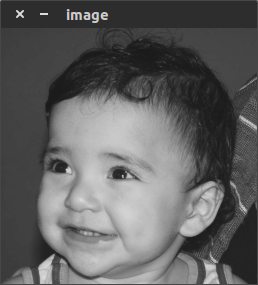
\includegraphics[width=2.5truein]{hello.png}
\caption{Saída do programa hello}

\end{figure}

Caso o programa funcione conforme o exemplo, provavelmente seu
ambiente de testes estará operacional para os exemplos do tutorial.


Neste tutorial, geralmente imagens armazenada no formato PNG serão
usadas. Este formato suporta representação de imagens de diversas
formas, como em tons de cinza, coloridas e preto-e-branco. Imagens em
outros formatos tais como JPEG podem oferecer algumas limitações para
os casos que serão abordados. Por exemplo, arquivos JPEG armazenam
apenas imagens em formato colorido e, durante a o processo de gravação
das imagens, o algoritmo de compressão com perdas pode modificar o
conteúdo da imagem original a ser gravada.


\hypertarget{x-manipulando-pixels-em-uma-imagem}{\chapter{Manipulando pixels em uma imagem}}
O objetivo dessa lição é mostra como manipular os pixels de uma
imagem, mudando a cor de uma pequena região retangular de uma imagem
fornecida para processamento.


Alguns conceitos importantes serão abordados neste contexto:


\begin{itemize}

\item Alguns tipos de dados comuns mais usados no OpenCV.

\item Funções para realizar entrada/saída de dados.

\item Funções para acessar os pixels de uma imagem.

\item Funções para realizar interações na interface gráfica.

\end{itemize}


Para evoluir nesses conceitos, realize o download do programa
\href{exemplos/pixels.cpp}{pixels.cpp}, mostrado na Listagem
\hyperlink{exa-pixels}{Pixels}, e a imagem \href{figs/bolhas.png}{bolhas.png}. Salve
ambos os arquivos que contém o \emph{Makefile}. O programa irá abrir a
imagem \texttt{bolhas.png} (interpretando-a em escala de cinza), deverá
exibi-la em uma janela e desenhar um quadrado preto em uma região
pré-estabelecida.


Após isso, ele irá aguardar que o usuário pressione alguma tecla. Uma
vez pressionada a tecla, o programa reabrirá o arquivo da imagem
interpretando-a em escala de cores e passará a desenhar um quadrado
vermelho na mesma região que foi pré-estabelecida.


\begin{verbatim}
#include <iostream>
#include <opencv2/opencv.hpp>

using namespace cv;
using namespace std;

int main(int, char**){
  Mat image;
  Vec3b val;

  image= imread("bolhas.png",CV_LOAD_IMAGE_GRAYSCALE);
  if(!image.data)
    cout << "nao abriu bolhas.png" << endl;

  namedWindow("janela",WINDOW_AUTOSIZE);

  for(int i=200;i<210;i++){
    for(int j=10;j<200;j++){
      image.at<uchar>(i,j)=0;
    }
  }

  imshow("janela", image);
  waitKey();

  image= imread("bolhas.png",CV_LOAD_IMAGE_COLOR);

  val[0] = 0;   //B
  val[1] = 0;   //G
  val[2] = 255; //R

  for(int i=200;i<210;i++){
    for(int j=10;j<200;j++){
      image.at<Vec3b>(i,j)=val;
    }
  }

  imshow("janela", image);
  waitKey();
  return 0;
}
\end{verbatim}

Para compilar e executar o programa
\href{exemplos/pixels.cpp}{pixels.cpp}, salve-o juntamente com o arquivo
\href{exemplos/Makefile}{Makefile} em um diretório e execute a seguinte
seqüência de comandos:


\begin{verbatim}
$ make pixels
$ ./pixels
\end{verbatim}

A saída do programa \emph{pixels} é mostrado na Figura \hyperlink{fig-pixels}{Pixels}


\begin{figure}[h]{}
\centering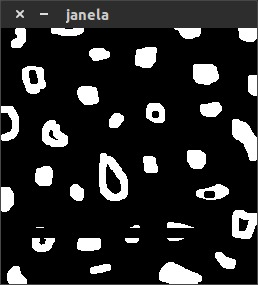
\includegraphics[width=2.5truein]{pixels.png}
\caption{Saída do programa pixels}

\end{figure}

\hypertarget{x-descrição-do-programa-\texttt{pixels.cpp}}{\section{Descrição do programa \texttt{pixels.cpp}}}
\begin{verbatim}
#include <iostream>
#include <opencv2/opencv.hpp>

using namespace cv;
using namespace std;
\end{verbatim}

Em geral, a maior parte das funcionalidades da biblioteca é definida
no arquivo de cabeçalho \texttt{opencv.hpp}. Nesse arquivo, são definidos
tipos básicos da biblioteca, bem como os protótipos de várias funções
usadas para tratamento de imagens. Ele agrega as definições de funções
que são usadas para entrada e saída de dados, criação de e manipulação
de janelas e seus eventos, além de \emph{widgets} para permitir interação
com o usuário.


Todas as clases e funções do OpenCV normalmente estão definidas no
\emph{namespace} \texttt{cv}. Portanto, declarar o uso do \emph{namespace} no início do
código pode ser conveniente para o programador. Isso evita que a
invocação das funções e tipos seja sempre precedido por \texttt{cv::}. A
convivência com o \emph{namespace} \texttt{std} geralmente é harmoniosa.


\begin{verbatim}
Mat image;
\end{verbatim}

A interface em C++ do OpenCV provê um tipo básico de estrutura para
armazenar imagems: a classe \texttt{Mat}. Dependendo da forma como é criado,
um objeto dessa classe é capaz de armazenar imagens (matrizes) de
diversos tipos diferentes, tais como inteiros, floats, doubles, etc.


Dezenas de métodos são providos para essa classe, métodos estes que
serão apresentados ao longo do tutorial, conforme a demanda se
dê. Nesta lição, apenas o método \texttt{at} será utilizado.


Outros tipos também são predefinidos no OpenCV, tal como o tipo
Vec3b. A classe \texttt{Vec} é definida no OpenCV para abrigar diversas
formas de vetores curtos. A classe é definida por gabaritos e provê
armazenamento de uma quantidade de valores de um dado tipo fornecido
na instanciação do gabarito.


Para ilustrar o uso da classe \texttt{Vec}, são mostrados em seguida, alguns
dos tipos predefinidos internamente no OpenCV.


\begin{verbatim}
typedef Vec<uchar, 2> Vec2b;
typedef Vec<uchar, 3> Vec3b;
typedef Vec<uchar, 4> Vec4b;

typedef Vec<short, 2> Vec2s;
typedef Vec<short, 3> Vec3s;
typedef Vec<short, 4> Vec4s;

typedef Vec<int, 2> Vec2i;
typedef Vec<int, 3> Vec3i;
typedef Vec<int, 4> Vec4i;

typedef Vec<float, 2> Vec2f;
typedef Vec<float, 3> Vec3f;
typedef Vec<float, 4> Vec4f;
typedef Vec<float, 6> Vec6f;

typedef Vec<double, 2> Vec2d;
typedef Vec<double, 3> Vec3d;
typedef Vec<double, 4> Vec4d;
typedef Vec<double, 6> Vec6d;
\end{verbatim}

Neste caso, o tipo Vec3b usado no exemplo representa um vetor de três
componentes, cada uma do tipo \texttt{unsigned char}, ocupando apenas um
byte na memória.


\begin{verbatim}
image= imread("bolhas.png",CV_LOAD_IMAGE_GRAYSCALE);
if(!image.data)
  cout << "nao abriu bolhas.png" << endl;
\end{verbatim}

Esse trecho de código usa a função \texttt{imread()} para ler uma imagem
presente em um arquivo e armazená-la no objeto \texttt{image}. A função
\texttt{imread()} recebe dois parâmetros: o primeiro é o caminho para o arquivo
a ser aberto; o segundo é a forma como a imagem será
interpretada. Neste casso, independentemente do formato da imagem
presente no arquivo \texttt{bolhas.png}, ela será imediatamente transformada
em uma imagem em tons de cinza antes de ser guardada no objeto
\texttt{image}.


Caso o arquivo não seja aberto (ex: o arquivo não foi encontrado, ou o
usuário não possui permissão de leitura ativado), o campo \texttt{data} do
objeto \texttt{image} deverá ter valor nulo, sinalizando o erro.


Algo importante a ser observado nesse momento é que, embora a
estrutura para armazenamento de imagens seja provida por uma classe -
a classe \texttt{Mat} - algumas das estruturas internas são públicas. Isso
ajuda a não haver degradação de desempenho com o uso excessivo de
chamadas de métodos.


\begin{verbatim}
namedWindow("janela", WINDOW_AUTOSIZE);
\end{verbatim}

Cria uma janela para que o usuário possa referenciá-la pelo nome que é
fornecido. O parâmetro \texttt{WINDOW_AUTOSIZE} permitirá que a janela se
ajuste automaticamente para o tamanho da imagen que for fornecida para
exibição.


\begin{verbatim}
for(int i=200;i<210;i++){
  for(int j=10;j<200;j++){
    image.at<uchar>(i,j)=0;
  }
}
\end{verbatim}

Este trecho de código desenha um retângulo preto na imagem. Neste
caso, assumindo que a primeira dimensão representa a coordenada \emph{x} e
a segunda dimensão da matriz representa a coordenada \emph{y}, será
desenhado um retângulo do ponto (200,10) até o ponto
(210,200).


Os pixels da região são acessados ou modificados com o método
\texttt{at}. Observe que este método sofre o efeito de um gabarito, que deve
receber um tipo correspondente o tipo de dado que está armazenado no
objeto \texttt{image}. Como a leitura foi feita assumindo uma imagem em tons
de cinza, o tipo de dado necessário será, neste caso, \texttt{unsigned
char}. Tipos diferentes poderão gerar resultados incorretos, posto que
a função \texttt{at()} interpretará a sequência de bytes da matriz \texttt{image} de
forma inapropriada.


Para manter os sistema referencial do tipo destrógiro, assume-se que
os eixos \emph{x} e \emph{y} ficarão organizados conforme apresenta a Figura
\hyperlink{fig-eixos}{Eixos}, com a origem no canto superior esquerdo da imagem.


\begin{figure}[h]{}
\centering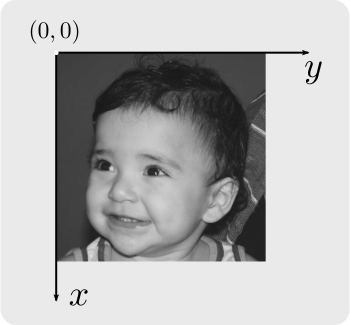
\includegraphics[width=2.5truein]{eixos.svg}
\caption{Sistema referencial adotado no OpenCV.}

\end{figure}

\begin{verbatim}
imshow("janela", image);
waitKey();
\end{verbatim}

A imagem \texttt{image} é mostrada na janela "\emph{janela}" e o programa aguarda
até que o usuário digite alguma tecla.


\begin{verbatim}
image= imread("bolhas.png",CV_LOAD_IMAGE_COLOR);
\end{verbatim}

O procedimento que segue repete os passos anteriores, só que agora a
imagem interpretada com três componentes de cor. A matriz \texttt{image}
agora guardará, para cada pixel, um conjunto de 3 bytes para armazenar
as contribuições de vermelho, verde e amarelo que este possui.


\begin{verbatim}
val[0] = 0;   //B
val[1] = 0;   //G
val[2] = 255; //R
\end{verbatim}

As cores em um pixel são ordenadas na sequência B->G->R (Azul, Verde,
Vermelho), podendo os pixels da matriz serem interpretados como um
conjunto de elementos do tipo \texttt{Vec3b}.


\begin{verbatim}
for(int i=200;i<210;i++){
  for(int j=10;j<200;j++){
    image.at<Vec3b>(i,j)=val;
  }
}
\end{verbatim}

Agora, a função \texttt{at()} interpreta a sequência de bytes usada para
armazenar a matriz \texttt{image} como sendo formadas por pixels do tipo
\texttt{Vec3b}, sendo às posições correspondentes atribuídas a cor vermelha
predefinida na variável \texttt{val}.


\hypertarget{x-exercícios}{\section{Exercícios}}
\begin{itemize}

\item Utilizando o programa \href{exemplos/pixels.cpp}{exemplos/pixels.cpp} como referência,
implemente um programa \texttt{regions.cpp}. Esse programa deverá solicitar
ao usuário as coordenadas de dois pontos P_1 e P_2
localizados dentro dos limites do tamanho da imagem e exibir que lhe
for fornecida. Entretanto, a região definida pelo retângulo de
vértices opostos definidos pelos pontos P_1 e P_2 será
exibida com o negativo da imagem na região correspondente. O efeito
é ilustrado na Figura \hyperlink{fig-regions}{Regiões}.

\end{itemize}


\begin{figure}[h]{}
\centering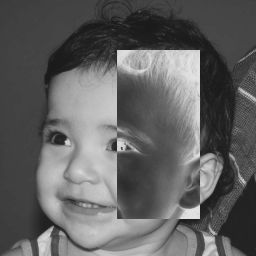
\includegraphics[width=2.5truein]{regions.png}
\caption{Exemplo de saída do programa regions.cpp}

\end{figure}

\begin{itemize}

\item Utilizando o programa \href{exemplos/pixels.cpp}{exemplos/pixels.cpp} como referência,
implemente um programa \texttt{trocaregioes.cpp}. Seu programa deverá
trocar os quadrantes em diagonal na imagem. Explore o uso da classe
\texttt{Mat} e seus construtores para criar as regiões que serão
trocadas. O efeito é ilustrado na Figura \hyperlink{fig-trocaregioes}{Troca de regiões}.

\end{itemize}


\begin{figure}[h]{}
\centering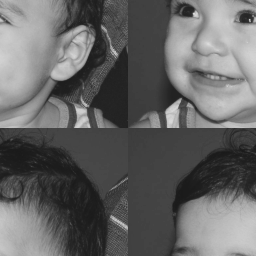
\includegraphics[width=2.5truein]{trocaregioes.png}
\caption{Exemplo de saída do programa trocaregioes.cpp}

\end{figure}

\hypertarget{x-preenchendo-regiões}{\chapter{Preenchendo regiões}}
Uma tarefa bastante comum em processamento de imagens e visão
artificial é contar a quantidade de objetos presentes em uma cena.


Para contar os objetos é necessário identificar os aglomerados de
pixels associados a cada um. Neste exemplo, assume-se que a imagem é
do tipo binária, ou seja, cada pixel assume apenas dois valores - 0 ou
255 - indicando que o pixel pertence ao fundo da imagem ("0") ou a
algum objeto presente ("255"). Assume-se também que cada aglomerado de
pixels será interpretado como um objeto individual. Esse é o processo
mais comum para operações de contagem de objetos em uma imagem.


Uma das maneiras de identificar as regiões de forma única é através de
rotulação. A rotulação de regiões é o processo pelo qual regiões com
características comuns recebem um identificador comum (rótulo).


Em geral, um algoritmo de rotulação de imagens binárias recebe como
entrada uma imagem binária e fornece como saída uma imagem em tons de
cinza, com as várias regiões representativas de objetos rotuladas com
um tom de cinza diferente.


No exemplo dessa lição será mostrado como rotular uma imagem binária,
utilizando o algoritmo \emph{floodfill} (ou \emph{seedfill}) para descobrir os
aglomerados de pixels. A imagem usada para teste será a presente no arquivo
\href{figs/bolhas.png}{bolhas.png} mostrada na Figura \hyperlink{fig-bolhas}{Bolhas}.


\begin{figure}[h]{}
\centering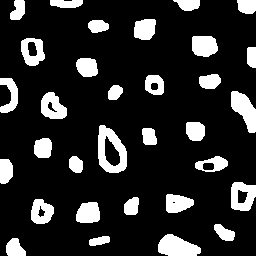
\includegraphics[width=2.5truein]{bolhas.png}
\caption{Imagem bolhas.png}

\end{figure}

O programa de referência utilizado para essa tarefa,
\href{exemplos/labeling.cpp}{labeling.cpp}, é mostrado na Listagem
\hyperlink{exa-labeling}{Labeling}.


\begin{verbatim}
#include <iostream>
#include <opencv2/opencv.hpp>

using namespace cv;

int main(int argc, char** argv){
  Mat image, mask;
  int width, height;
  int nobjects;

  CvPoint p;
  image = imread(argv[1],CV_LOAD_IMAGE_GRAYSCALE);

  if(!image.data){
    std::cout << "imagem nao carregou corretamente\n";
    return(-1);
  }
  width=image.size().width;
  height=image.size().height;

  p.x=0;
  p.y=0;

  // busca objetos com buracos presentes
  nobjects=0;
  for(int i=0; i<height; i++){
    for(int j=0; j<width; j++){
      if(image.at<uchar>(i,j) == 255){
		// achou um objeto
		nobjects++;
		p.x=j;
		p.y=i;
		floodFill(image,p,nobjects);
	  }
	}
  }
  imshow("image", image);
  imwrite("labeling.png", image);
  waitKey();
  return 0;
}
\end{verbatim}

Para compilar e executar o programa \href{exemplos/labeling.cpp}{labeling.cpp},
salve-o juntamente com os arquivo \href{exemplos/Makefile}{Makefile} e
\href{figs/bolhas.png}{bolhas.png} em um diretório e execute a seguinte seqüência de comandos:


\begin{verbatim}
$ make labeling
$ ./labeling bolhas.png
\end{verbatim}

A saída do programa \emph{labeling} é mostrado na Figura \hyperlink{fig-labeling}{Labeling}


\begin{figure}[h]{}
\centering
\includegraphics[width=2.5truein]{labeling.png}
\caption{Saída do programa labeling}

\end{figure}

\hypertarget{x-descrição-do-programa-\texttt{labeling.cpp}}{\section{Descrição do programa \texttt{labeling.cpp}}}
\begin{verbatim}
CvPoint p;
\end{verbatim}

A estrutura \texttt{CvPoint} define um ponto na segunda dimensão que permite
acesso às suas coordenadas x e y. Ele será usado no exemplo para
indicar a semente de preenchimento que é usada pelo algoritmo \emph{floodfill}.


\begin{verbatim}
image = imread(argv[1],CV_LOAD_IMAGE_GRAYSCALE);
\end{verbatim}

Independentemente do formato da imagem de entrada, ela será convertida
para tons de cinza, uma vez que o exemplo assume essa condição.


\begin{verbatim}
p.x=0;
p.y=0;
\end{verbatim}

Nesta fase tem início o processo de rotulação das várias regiões da
imagem. Assumindo que os pixels do objeto possuem tom de cinza igual a
255, o algoritmo percorre toda a imagem, linha após linha, de cima a
baixo, da esquerda para direita por pixels que tenham tom igual
a 255.


Quando um elemento da matriz é encontrado com tom de cinza igual a
255, o algoritmo \emph{floodfill} é executado utilizando as coordenadas
desse ponto como semente.


A operação do algoritmo \emph{floodfill} é bem simples: dado um ponto
semente, o algoritmo sai procurando os 4- ou 8-vizinhos desse ponto
(conforme configuração estabelecida) que possuem a mesma propriedade
do ponto semente (geralmente o tom de cinza). Para cada ponto
encontrado, muda-se sua propriedade para uma nova propriedade
fornecida. Para cada ponto encontrado, também, realiza-se a busca de
vizinhança para os seus 4- ou 8-vizinhos que contenham a mesma
propriedade da semente. Esse processo é repetido até que não restem
mais pontos com propriedade alterada na componente conectada (ou
região conectada).


\begin{verbatim}
nobjects=0;
\end{verbatim}

Inicia a contagem de objetos (inicialmente, zero objetos estão
presentes)


\begin{verbatim}
for(int i=0; i<height; i++){
  for(int j=0; j<width; j++){
    if(image.at<uchar>(i,j) == 255){
      nobjects++;
      p.x=j;
      p.y=i;
      floodFill(image,p,nobjects);
    }
  }
}
\end{verbatim}

A contagem funciona percorrendo as linhas e colunas da matriz \texttt{image}
em busca de elementos com tom de cinza igual a \texttt{255} (pixel de
objeto). Quando encontrado, incrementa-se o contador de objeto e
executa-se o algoritmo \emph{floodfill} na imagem utilizando o pixel
encontrado como semente. Observe que a região à qual o pixel pertence
será rotulada com tom de cinza igual ao número de contagem de objetos
atual.


O processo continua até que toda a imagem tenha sido rotulada.


\begin{verbatim}
imshow("image", image);
imwrite("labeling.png", image);
waitKey();
\end{verbatim}

Finalmente, a imagem \texttt{image} é mostrada (já completamente rotulada) e
então gravada no arquivo \texttt{labeling.png}.


\hypertarget{x-exercícios}{\section{Exercícios}}
\begin{itemize}

\item Observando-se o programa \href{exemplos/labeling.cpp}{labeling.cpp} como
exemplo, é possível verificar que caso existam mais de 255 objetos
na cena, o processo de rotulação poderá ficar
comprometido. Identifique a situação em que isso ocorre e proponha
uma solução para este problema.

\item Aprimore o algoritmo de contagem apresentado para identificar
regiões com ou sem buracos internos que existam na cena. Assuma que
objetos com mais de um buraco podem existir. Inclua suporte no seu
algoritmo para não contar bolhas que tocam as bordas da imagem. Não
se pode presumir, a priori, que elas tenham buracos ou não.

\end{itemize}


\hypertarget{x-manipulação-de-histogramas}{\chapter{Manipulação de histogramas}}
O objetivo dessa lição é mostrar como tratar histogramas de imagens usando
OpenCV. Histogramas são ferramentas interessantes para avaliar
características de uma imagem ou de atributos que dela são extraídos.


Um histograma é uma contagem de dados onde se organiza as ocorrências
por faixas de valores predefinidos. Em se tratando de imagens digitais
em tons de cinza, por exemplo, costuma-se associar um histograma com a
contagem de ocorrências de cada um dos possíveis tons em uma imagem. A
grosso modo, o histograma oferece uma estimativa da probabilidade de
ocorrência dos tons de cinza na imagem.


Exemplos típicos do uso de histogramas podem ser encontrados na
segmentação automática de imagens, detecção de movimento e
granulometria.


Além disso, a lição deverá explorar o uso dos recursos de captura de
vídeo disponíveis no OpenCV para lidar com câmeras conectadas ao
sistema.


O exemplo da Listagem \hyperlink{exa-histogram}{Histograma} mostra o processo de capturar
imagens de uma \emph{webcam} instalada no computador, calcular os
histogramas das componentes de cor das imagens e desenhá-los no canto
superior esquerdo da imagem capturada.


\begin{verbatim}
#include <iostream>
#include <opencv2/opencv.hpp>

using namespace cv;
using namespace std;

int main(int argc, char** argv){
  Mat image;
  int width, height;
  VideoCapture cap;
  vector<Mat> planes;
  Mat histR, histG, histB;
  int nbins = 64;
  float range[] = {0, 256};
  const float *histrange = { range };
  bool uniform = true;
  bool acummulate = false;

  cap.open(0);

  if(!cap.isOpened()){
    cout << "cameras indisponiveis";
    return -1;
  }

  width  = cap.get(CV_CAP_PROP_FRAME_WIDTH);
  height = cap.get(CV_CAP_PROP_FRAME_HEIGHT);

  cout << "largura = " << width << endl;
  cout << "altura  = " << height << endl;

  int histw = nbins, histh = nbins/2;
  Mat histImgR(histh, histw, CV_8UC3, Scalar(0,0,0));
  Mat histImgG(histh, histw, CV_8UC3, Scalar(0,0,0));
  Mat histImgB(histh, histw, CV_8UC3, Scalar(0,0,0));

  while(1){
    cap >> image;
    split (image, planes);
    calcHist(&planes[0], 1, 0, Mat(), histR, 1,
             &nbins, &histrange,
             uniform, acummulate);
    calcHist(&planes[1], 1, 0, Mat(), histG, 1,
             &nbins, &histrange,
             uniform, acummulate);
    calcHist(&planes[2], 1, 0, Mat(), histB, 1,
             &nbins, &histrange,
             uniform, acummulate);

    normalize(histR, histR, 0, histImgR.rows, NORM_MINMAX, -1, Mat());
    normalize(histG, histG, 0, histImgG.rows, NORM_MINMAX, -1, Mat());
    normalize(histB, histB, 0, histImgB.rows, NORM_MINMAX, -1, Mat());

    histImgR.setTo(Scalar(0));
    histImgG.setTo(Scalar(0));
    histImgB.setTo(Scalar(0));

    for(int i=0; i<nbins; i++){
      line(histImgR,
           Point(i, histh),
           Point(i, histh-cvRound(histR.at<float>(i))),
           Scalar(0, 0, 255), 1, 8, 0);
      line(histImgG,
           Point(i, histh),
           Point(i, histh-cvRound(histG.at<float>(i))),
           Scalar(0, 255, 0), 1, 8, 0);
      line(histImgB,
           Point(i, histh),
           Point(i, histh-cvRound(histB.at<float>(i))),
           Scalar(255, 0, 0), 1, 8, 0);
    }
    histImgR.copyTo(image(Rect(0, 0       ,nbins, histh)));
    histImgG.copyTo(image(Rect(0, histh   ,nbins, histh)));
    histImgB.copyTo(image(Rect(0, 2*histh ,nbins, histh)));
    imshow("image", image);
    if(waitKey(30) >= 0) break;
  }
  return 0;
}
\end{verbatim}

Para compilar e executar o programa
\href{exemplos/histogram.cpp}{histogram.cpp}, salve-o juntamente com o arquivo
\href{exemplos/Makefile}{Makefile} em um diretório e execute a seguinte
seqüência de comandos:


\begin{verbatim}
$ make histogram
$ ./histogram
\end{verbatim}

A saída do programa \emph{histogram} é mostrado na Figura \hyperlink{fig-histogram}{Histogram}


\begin{figure}[h]{}
\centering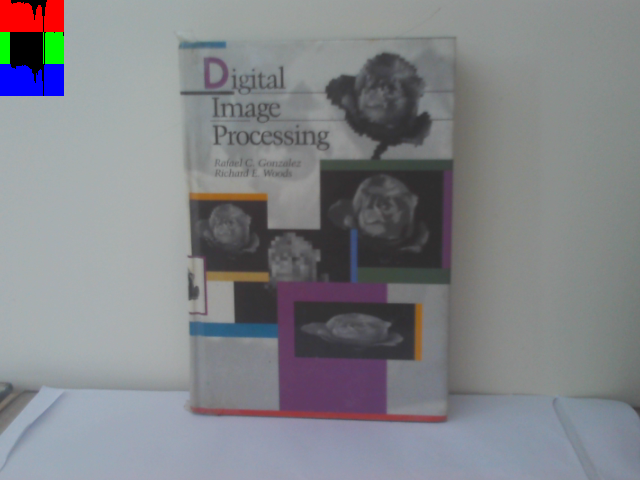
\includegraphics[width=2.5truein]{histogram.png}
\caption{Saída do programa histogram}

\end{figure}

\hypertarget{x-descrição-do-programa-\texttt{histogram.cpp}}{\section{Descrição do programa \texttt{histogram.cpp}}}
\begin{verbatim}
VideoCapture cap;
\end{verbatim}

Fontes de captura de vídeo são acessadas no OpenCV através da classe
\texttt{VideoCapture}. Com ela, o usuário pode abrir um fluxo de vídeo
oriundo de um arquivo de vídeo, sequência de imagens ou de um
dispositivo de captura. Neste último caso, os dispositivos são
identificados por um índice que inicia em \texttt{0}.


As imagens capturadas nesse exemplo serão extraídas de um fluxo de
vídeo que será conectado ao objeto \texttt{cap}.


\begin{verbatim}
vector<Mat> planes;
Mat histR, histG, histB;
int nbins = 64;
\end{verbatim}

O cálculo do histograma será realizado para cada uma das componentes
de cor de forma independente. Logo, a separação das componentes em
matrizes independentes será feita no vetor de matrizes
\texttt{planes}. Assim, \texttt{planes[0]}, \texttt{planes[1]} e \texttt{planes[2]} armazenarão as
componentes de cor Vermelho, Verde e Azul, respectivamente.


As três matrizes \texttt{histR}, \texttt{histG} e \texttt{histB} guardarão os histogramas
de suas respectivas componentes de cor.


A variável \texttt{nbins} define o tamanho do vetor utilizado para armazenar
os histogramas. O tamanho do histograma não precisa ser
necessariamente o mesmo do ton de cinza máximo previsto para uma
componente de cor (ex: 256 para imagens RGB). É possível especificar a
quantidade de faixas (ou \emph{bins}) que serão usadas para quantificar
as ocorrências dos tons.


No exemplo, usa-se um total de 64 faixas para um tom de cinza máximo
igual a 255. No cálculo, portanto, as ocorrências de tom de cinza na
faixa [0,3] serão contabilizadas no primeiro elemento do array
com o histograma; as ocorrências na faixa [4,7] contarão no
segundo elemento do histograma, e assim por diante.


\begin{verbatim}
float range[] = {0, 256};
const float *histrange = { range };
\end{verbatim}

É preparada na variável \texttt{histrange} a faixa de valores (mínimo e
máximo) presentes na imagem cujo histograma será calculado. Essa
variável, da forma como é definida, é usada pela função de cálculo de
histograma.


\begin{verbatim}
bool uniform = true;
bool acummulate = false;
\end{verbatim}

\begin{verbatim}
cap.open(0);

if(!cap.isOpened()){
  cout << "cameras indisponiveis";
  return -1;
}

width  = cap.get(CV_CAP_PROP_FRAME_WIDTH);
height = cap.get(CV_CAP_PROP_FRAME_HEIGHT);
\end{verbatim}

Abre-se a conexão com o primeiro dispositivo de captura de vídeo
disponível. Os dispositivos são identificados em sequência. Logo, se
um sistema dispõe de duas câmeras, por exemplo, a primeira será
associada ao identificador "0" e a segunda ao identificador "1".


Uma vez chamado o método \texttt{open()}, verifica-se se o dispositivo de
captura está devidamente conectado para proceder com o restante das
tarefas.


Finalmente, lê-se a largura (\emph{width}) e altura(\emph{height}) dos quadros
que serão disponíveis pelo dispositivo. A classe \texttt{VideoCapture} possui
diversos métodos para ajustar os parâmetros de captura para o
dispositivo conectado. Entretanto, na versão do OpenCV em que foram
feitos os testes aqui descritos, alguns podem não funcionar
corretamente dependendo do tipo de dispositivo utilizado.


\begin{verbatim}
int histw = nbins, histh = nbins/2;
Mat histImgR(histh, histw, CV_8UC3, Scalar(0,0,0));
Mat histImgG(histh, histw, CV_8UC3, Scalar(0,0,0));
Mat histImgB(histh, histw, CV_8UC3, Scalar(0,0,0));
\end{verbatim}

Define-se a largura e altura das imagens que serão usadas para
desenhar os histogramas de cada uma das componentes de cor. Note que a
altura da imagem é igual à metade da largura para fins de exibição. As
imagens são criadas com o tipo \texttt{CV_8UC3}, ou seja, com 8 bits por
pixel, com tipo de dados \texttt{unsigned char} contendo 3 canais de cor. A
cor, nesse caso, servirá apenas para que o histograma seja desenhado
na cor respectiva de sua componente.


\begin{verbatim}
cap >> image;
split (image, planes);
\end{verbatim}

Em um loop infinito, as imagens são capturadas, quadro a quadro, do
dispositivo de entrada conectado e armazenadas no objeto
\texttt{image}. Dispositivos de captura normalmente disponibilizam imagens
com suporte a cor, ou seja, cada matriz possui normalmente três planos
de cor. Logo, os histogramas deverão ser calculados para cada um
desses planos, de modo que a função \texttt{split()} faz a separação adequada
para que se proceda com o cálculo.


Histogramas hiperdimensionais que contabilizam as ocorrências das
combinações R,G e B dos pixels de uma imagem são possíveis de serem
calculados. Entretanto, normalmente são usadas matrizes esparças para
isso. Considerando imagens com 8 bits por pixel para cada plano de
cor, seria necessário uma matriz com 256 x 256 x 256 elementos para
guardar o histograma até mesmo de uma imagem pequena. Esse processo é
dispendioso e, normalmente, não possui muita utilidade.


Na análise de histograma, portanto, geralmente se avalia cada
componente de cor de forma independente.


\begin{verbatim}
calcHist(&planes[0], 1, 0, Mat(), histR, 1,
         &nbins, &histrange,
         uniform, acummulate);
calcHist(&planes[1], 1, 0, Mat(), histG, 1,
         &nbins, &histrange,
         uniform, acummulate);
calcHist(&planes[2], 1, 0, Mat(), histB, 1,
         &nbins, &histrange,
         uniform, acummulate);
\end{verbatim}

Os histogramas são então calculados para cada uma das componentes
de cor. A função \texttt{calcHist()} do OpenCV recebe, na sequência, os
seguintes argumentos:


\begin{itemize}

\item Uma referência para imagem que se deseja processar;

\item A quantidade de imagens para se calcular o histograma (uma, neste
caso);

\item Um ponteiro para o array de canais das imagens. Para apenas um
canal, o endereço \texttt{0} deve ser repassado;

\item Uma máscara opcional marcando a região onde se deseja calcular o
histograma. Considerando a imagem inteira, fornece-se uma matriz
vazia;

\item O array que irá armazenar o histograma;

\item A dimensionalidade do histograma (no exemplo, existe apenas uma
dimensão);

\item O endereço da variável que armazena a quantidade de divisões; e

\item Variáveis informando se o histograma é uniforme (divisões de tamanho
igual) ou acumulado.

\end{itemize}


\begin{verbatim}
normalize(histR, histR, 0, histImgR.rows, NORM_MINMAX, -1, Mat());
normalize(histG, histB, 0, histImgR.rows, NORM_MINMAX, -1, Mat());
normalize(histB, histB, 0, histImgR.rows, NORM_MINMAX, -1, Mat());
\end{verbatim}

Cada histograma é normalizado em uma faixa de valores que vai de \texttt{0}
até a quantidade de linhas da imagem onde este será desenhado. A
normalização é feita linearmente entre os valores máximo e mínimo
encontrados na componente de cor.


\begin{verbatim}
histImgR.setTo(Scalar(0));
histImgG.setTo(Scalar(0));
histImgB.setTo(Scalar(0));

for(int i=0; i<nbins; i++){
  line(histImgR, Point(i, histh),
       Point(i, cvRound(histR.at<float>(i))),
       Scalar(0, 0, 255), 1, 8, 0);
  line(histImgG, Point(i, histh),
       Point(i, cvRound(histG.at<float>(i))),
       Scalar(0, 255, 0), 1, 8, 0);
  line(histImgB, Point(i, histh),
       Point(i, cvRound(histB.at<float>(i))),
       Scalar(255, 0, 0), 1, 8, 0);
}
\end{verbatim}

As imagens com os desenhos dos histogramas são então
geradas. Inicialmente, todas são preenchidas com \texttt{0} (cor preta). Em
seguida, os histogramas são desenhados na forma de um gráfico de
barras usando a função \texttt{line()}.


\begin{verbatim}
histImgR.copyTo(image(Rect(0, 0       ,nbins, histh)));
histImgG.copyTo(image(Rect(0, histh   ,nbins, histh)));
histImgB.copyTo(image(Rect(0, 2*histh ,nbins, histh)));
\end{verbatim}

Finalmente, as imagens dos histogramas são copiadas, uma abaixo da
outra, para o canto superior esquerdo da imagem capturada na câmera.


\hypertarget{x-exercícios}{\section{Exercícios}}
\begin{itemize}

\item Utilizando o programa \href{exemplos/histogram.cpp}{exemplos/histogram.cpp} como referência,
implemente um programa \texttt{equalize.cpp}. Este deverá, para cada
imagem capturada, realizar a equalização do histogram antes de
exibir a imagem. Teste sua implementação apontando a câmera para
ambientes com iluminações variadas e observando o efeito
gerado. Assuma que as imagens processadas serão em tons de cinza.

\item Utilizando o programa \href{exemplos/histogram.cpp}{exemplos/histogram.cpp} como referência,
implemente um programa \texttt{motiondetector.cpp}. Este deverá
continuamente calcular o histograma da imagem (apenas uma componente
de cor é suficiente) e compará-lo com o último histograma
calculado. Quando a diferença entre estes ultrapassar um limiar
pré-estabelecido, ative um alarme. Utilize uma função de comparação
que julgar conveniente.

\end{itemize}


\hypertarget{x-filtragem-no-domínio-espacial-i}{\chapter{Filtragem no domínio espacial I}}
A convolução é um processo pelo qual duas funções se combinam para
formar uma terceira função no domínio espacial. Tal processo resulta
do deslocamento de uma função sobre a outra e do cálculo de uma
combinação linear entre ambas em cada ponto do deslocamento.


Em se tratando de uma imagem digital, a convolução é chamada de
convolução digital. Sua principal aplicação é na filtragem de sinais,
permitindo que características de uma dada imagem sejam alteradas
conforme o tipo de efeito que se deseja impor.


A convolução discreta entre duas imagens pode ser definida como


h(x,y) = f(x,y)*g(x,y) = \frac{1}{MN}
\sum_{m=0}^{M-1}\sum_{n=0}^{N-1}f(m,n) g(x-m, y-n)


As funções f(x,y) e g(x,y) normalmente estão associadas
à imagem a ser filtrada e ao filtro digital associado.


Existem dois tipos de convolução: a 'convolução linear' e a
'convolução circular'. Na primeira, assume-se que os sinais
f(x,y) e g(x,y) existem em duas regiões com M e N
amostras consecutivas, respectivamente, sendo zero fora desssas
regiões. A região resultante da convolução terá suporte de tamanho
M+N-1. Fora desta, o resultado da convolução será nulo. Na
segunda, assume-se que as sequências f(x,y) e g(x,y) são
periódicas e com um mesmo período M=N. O resultado da
convolução, h(x,y) possuirá também o mesmo período M.


Costuma-se simplificar essa equação e calcular os tons de cinza da
imagem filtrada realizando o produto entre os coeficientes de uma
pequena matriz comumente denominada 'máscara' e as intensidades dos
pixels sobre uma posição específica na imagem.


As máscaras normalmente possuem dimensões de tamanho ímpar (3
\times 3 elementos , 5 \times 5 elementos, 7 \times 7
elementos, etc), dependendo da intensidade da filtragem que se deseja
realizar.


Considere uma imagem digital denotada por f(x,y), uma matriz de
máscara denotada por w(s,t) e uma image filtrada denotada por
g(x,y). Para uma máscara de tamanho 3 \times 3
elementos, o processo de filtragem no domínio espacial é ilustrado na
figura \hyperlink{fig-filtragemespacial}{Filtragem espacial}.


\begin{figure}[h]{}
\centering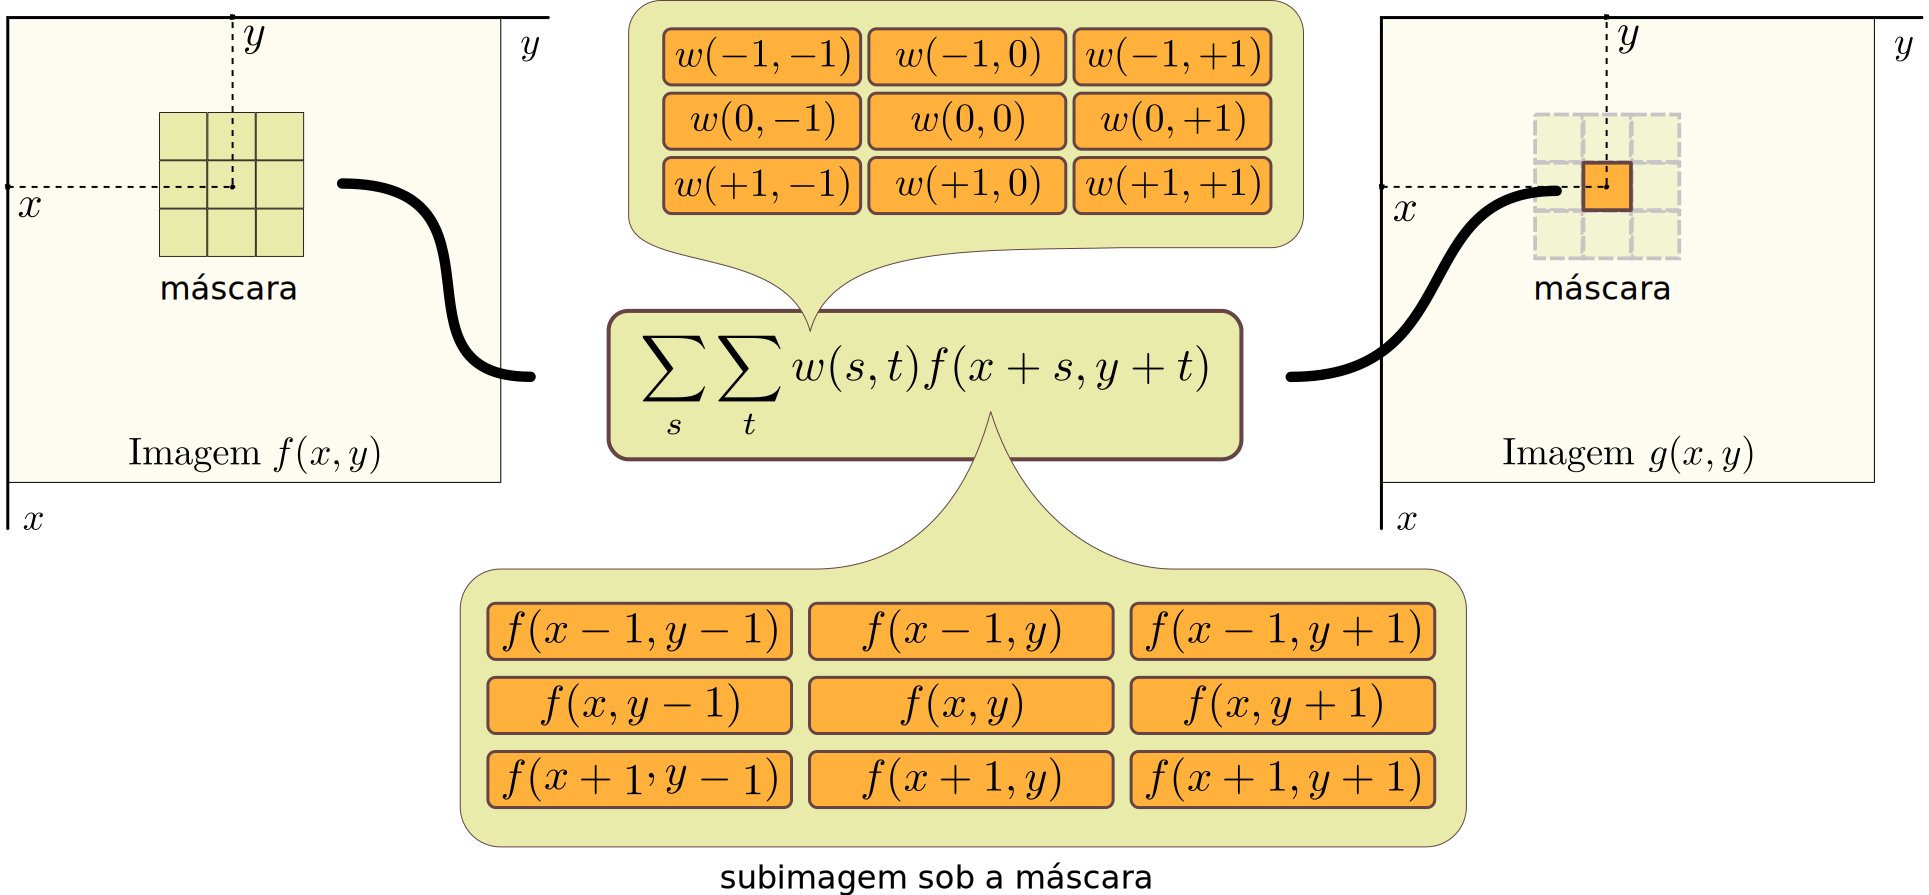
\includegraphics[width=2.5truein]{filtragemespacial.svg}
\caption{Filtragem espacial}

\end{figure}

No processo, a imagem da máscara é deslocada (pixel a pixel) sobre a
imagem a ser filtrada. Para cada deslocamento, calcula-se o somatório
do produto entre os valores dos elementos da máscara e os tons de
cinza dos pixels que esta sobrepõe e atribui-se o resultado ao pixel
respectivo na imagem filtrada.


Muitos efeitos de filtragem são possíveis de se obter modificando os
valores da imagem da máscara: borramento, aguçamento e detecção de
bordas são os principais deles.


O programa de referência utilizado para essa tarefa,
\href{exemplos/filtroespacial.cpp}{filtroespacial.cpp}, é mostrado na
Listagem \hyperlink{exa-filtroespacial}{Filtroespacial}.


\begin{verbatim}
#include <iostream>
#include <opencv2/opencv.hpp>

using namespace cv;
using namespace std;

void printmask(Mat &m){
  for(int i=0; i<m.size().height; i++){
    for(int j=0; j<m.size().width; j++){
      cout << m.at<float>(i,j) << ",";
    }
    cout << endl;
  }
}

void menu(){
  cout << "\npressione a tecla para ativar o filtro: \n"
	"a - calcular modulo\n"
    "m - media\n"
    "g - gauss\n"
    "v - vertical\n"
	"h - horizontal\n"
    "l - laplaciano\n"
	"esc - sair\n";
}

int main(int argvc, char** argv){
  VideoCapture video;
  float media[] = {1,1,1,
				   1,1,1,
				   1,1,1};
  float gauss[] = {1,2,1,
				   2,4,2,
				   1,2,1};
  float horizontal[]={-1,0,1,
					  -2,0,2,
					  -1,0,1};
  float vertical[]={-1,-2,-1,
					0,0,0,
					1,2,1};
  float laplacian[]={0,-1,0,
					 -1,4,-1,
					 0,-1,0};

  Mat cap, frame, frame32f, frameFiltered;
  Mat mask(3,3,CV_32F), mask1;
  Mat result, result1;
  double width, height, min, max;
  int absolut;
  char key;

  video.open(0);
  if(!video.isOpened())
    return -1;
  width=video.get(CV_CAP_PROP_FRAME_WIDTH);
  height=video.get(CV_CAP_PROP_FRAME_HEIGHT);
  std::cout << "largura=" << width << "\n";;
  std::cout << "altura =" << height<< "\n";;

  namedWindow("filtroespacial",1);

  mask = Mat(3, 3, CV_32F, media);
  scaleAdd(mask, 1/9.0, Mat::zeros(3,3,CV_32F), mask1);
  swap(mask, mask1);
  absolut=1; // calcs abs of the image

  menu();
  for(;;){
    video >> cap;
    cvtColor(cap, frame, CV_BGR2GRAY);
    flip(frame, frame, 1);
    imshow("original", frame);
    frame.convertTo(frame32f, CV_32F);
    filter2D(frame32f, frameFiltered, frame32f.depth(), mask, Point(1,1), 0);
    if(absolut){
      frameFiltered=abs(frameFiltered);
    }
    frameFiltered.convertTo(result, CV_8U);
    imshow("filtroespacial", result);
    key = (char) waitKey(10);
    if( key == 27 ) break; // esc pressed!
    switch(key){
    case 'a':
	  menu();
      absolut=!absolut;
      break;
    case 'm':
	  menu();
      mask = Mat(3, 3, CV_32F, media);
      scaleAdd(mask, 1/9.0, Mat::zeros(3,3,CV_32F), mask1);
      mask = mask1;
      printmask(mask);
      break;
    case 'g':
	  menu();
      mask = Mat(3, 3, CV_32F, gauss);
      scaleAdd(mask, 1/16.0, Mat::zeros(3,3,CV_32F), mask1);
      mask = mask1;
      printmask(mask);
      break;
    case 'h':
	  menu();
      mask = Mat(3, 3, CV_32F, horizontal);
      printmask(mask);
      break;
    case 'v':
	  menu();
      mask = Mat(3, 3, CV_32F, vertical);
      printmask(mask);
      break;
    case 'l':
	  menu();
      mask = Mat(3, 3, CV_32F, laplacian);
      printmask(mask);
      break;
    default:
      break;
    }
  }
  return 0;
}
\end{verbatim}

Para compilar e executar o programa \href{exemplos/filtroespacial.cpp}{filtroespacial.cpp},
salve-o juntamente com o arquivo \href{exemplos/Makefile}{Makefile}
em um diretório e execute a seguinte seqüência de comandos:


\begin{verbatim}
$ make filtroespacial
$ ./filtroespacial
\end{verbatim}

A saída do programa \emph{filtroespacial} apresentará duas janelas: uma com
a imagem original capturada e outra com o resultado da filtragem. O
filtro inicial escolhido no exemplo é o da média.


\hypertarget{x-descrição-do-programa-\texttt{filtroespacial.cpp}}{\section{Descrição do programa \texttt{filtroespacial.cpp}}}
\begin{verbatim}
float media[] = {1,1,1,
                 1,1,1,
                 1,1,1};
float gauss[] = {1,2,1,
                 2,4,2,
                 1,2,1};
float horizontal[]={-1,0,1,
                    -2,0,2,
                    -1,0,1};
float vertical[]={-1,-2,-1,
                  0,0,0,
                  1,2,1};
float laplacian[]={0,-1,0,
                   -1,4,-1,
                   0,-1,0};
\end{verbatim}

Os filtros usados no exemplo (determinados pelas matrizes de máscara)
são de tamanho 3 \times 3 pixels. Cinco tipos de filtros são
testados: média, gaussiano, detector de bordas horizontais, detector de
bordas verticais e laplaciano. Os coeficientes de cada filtro são
armazenados em arrays unidimensionais que serão repassados ao
construtor da matriz do filtro.


\begin{verbatim}
mask = Mat(3, 3, CV_32F, media);
scaleAdd(mask, 1/9.0, Mat::zeros(3,3,CV_32F), mask1);
swap(mask, mask1);
\end{verbatim}

Esse trecho de código mostra o procedimento padrão para construção da
matriz que será usada como máscara de filtragem. A variável \texttt{mask}
recebe uma matriz de tamanho 3 \times 3 em ponto flutuante
(\texttt{CV_32F}) com valores iniciais iguais ao do array \texttt{media} que é
repassado. Repare que o tipo da matriz precisa ser estabelecido em
ponto flutuante, posto que as operações de cálculo contarão com a
presença de números fracionários.


O uso da função \texttt{scaleAdd()} serve para dar o ganho de 1/9 nos
coeficientes do filtro da média. A operação multiplica o primeiro
argumento pelo segundo, soma com o terceiro argumento (neste caso, uma
matriz de zeros) e armazena o resultado no terceiro argumento,
\texttt{mask1}. Logo em seguida, a troca entre as matrizes \texttt{mask} e \texttt{mask1}
ocorre para que use apenas a matriz \texttt{mask} no cálculo da convolução
digital.


\begin{verbatim}
video >> cap;
cvtColor(cap, frame, CV_BGR2GRAY);
flip(frame, frame, 1);
\end{verbatim}

Em loop infinito, imagens coloridas são capturadas constantemente na
matriz \texttt{cap} e convertidas em equivalentes em tons de cinza usando a
função \texttt{cvtColor()}. A imagem então é invertida horizontalmente com a
função \texttt{flip()}. A inversão é feita apenas para fins de tornar a
interação com o programa exemplo semelhante à de um espelho.


\begin{verbatim}
frame.convertTo(frame32f, CV_32F);
filter2D(frame32f, frameFiltered, frame32f.depth(), mask, Point(1,1), 0);
\end{verbatim}

Este trecho é responsável pelo cálculo da filtragem espacial. Cada
imagem em tom de cinza armazenada na variável \texttt{frame} é convertida
para outra equivalente com representação em ponto flutuante -
\texttt{frame32f}. A conversão é necessária devido aos tipos de operação que
serão realizados pela função \texttt{filter2D()}. Observe apenas que OpenCV
replica os pixels na borda ('ao invés de preencher de zeros') durante
o processo de filtragem.


A função \texttt{filter2d()} recebe então a matriz da imagem em ponto
flutuante - \texttt{frame32f} - e produz a matriz \texttt{frameFiltered}, de acordo
com o tipo do elemento da matriz de entrada - neste caso, CV_32F (ou
float). O objeto \texttt{Point(1,1)} que é repassado como próximo argumento
identifica a origem do sistema de coordenadas atribuído para a
máscara que, neste caso, é o ponto central da matriz.


\begin{verbatim}
if(absolut){
  frameFiltered=abs(frameFiltered);
}
frameFiltered.convertTo(result, CV_8U);
\end{verbatim}

Caso a opção de módulo esteja selecionada, o cálculo é então
procedido. A imagem filtrada é então convertida para tons de cinza
para posterior exibição na tela.


O restante do código trata apenas da adaptação da matriz \texttt{mask}
conforme o filtro escolhido pelo usuário para ser aplicado à imagem
capturada.


\hypertarget{x-exercícios}{\section{Exercícios}}
\begin{itemize}

\item Utilizando o programa \href{exemplos/filtroespacial.cpp}{exemplos/filtroespacial.cpp} como
referência, implemente um programa \texttt{laplgauss.cpp}. O programa
deverá acrescentar mais uma funcionalidade ao exemplo fornecido,
permitindo que seja calculado o laplaciano do gaussiano das imagens
capturadas. Compare o resultado desse filtro com a simples aplicação
do filtro laplaciano.

\end{itemize}


\hypertarget{x-filtragem-no-domínio-espacial-ii}{\chapter{Filtragem no domínio espacial II}}
Este capítulo visa explorar um pouco mais do uso de filtragem espacial
aplicando seus princípios para simular uma técnica de fotografia denominada
\emph{tilt-shift}.


A técnica fotográfica de \emph{tilt-shift} envolve o uso de deslocamentos e
rotações entre a lente e o plano de projeção (onde fica filme
fotográfico ou o sensor da câmera) de modo a desfocar seletivamente
regiões do assunto.


O princípio básico dessa técnica é ilustrado na figura
\hyperlink{fig-tiltshift}{Tilt-shift}.


\begin{figure}[h]{}
\centering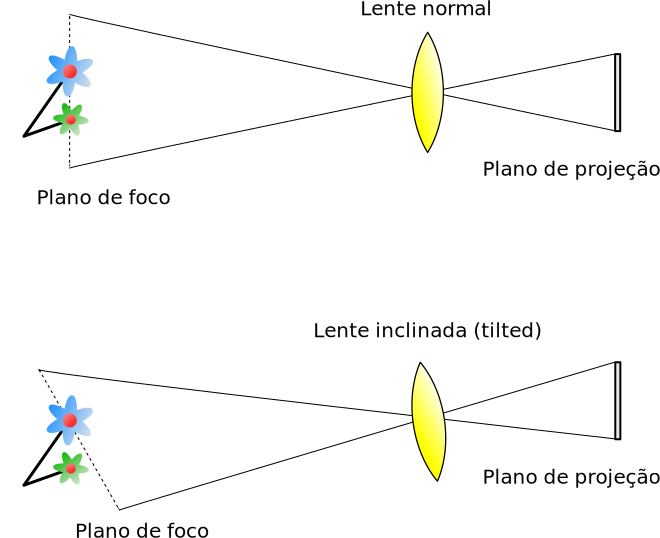
\includegraphics[width=2.5truein]{tiltshift.svg}
\caption{Princípio de funcionamento do _tilt shift_}

\end{figure}

Na lente normal, o plano de projeção é paralelo ao plano de foco com o
assunto que se deseja registrar. Quando a lente é submetida a uma
inclinação (\emph{tilt}), o plano de foco forma um ângulo diferente de zero
com o plano de projeção, mudando assim a região que ficará em foco na
imagem registrada pela câmera. Se a lente for deslocada para cima ou
para baixo (\emph{shift}), é possível também escolher seletivamente a
região que ficará em foco, complementando o uso da técnica.


A técnica de \emph{tilt-shift} consegue criar belos efeitos fotográficos,
simulando miniaturas. O foco seletivo que a lente produz engana o olho
humano, dando a impressão que a imagem foi registrada de uma cena em
miniatura. Tomando a imagem usando ângulos e proporções adequadas do
assunto, dá para se produzir versões em minatura de cenas reais que
podem ser bastante convincentes.


Lentes que produzem esse efeito não são baratas quando comparadas a
lentes normais. Entrentanto, o efeito produzido por estas lentes pode
ser reproduzido usando técnicas simples de processamento digital de
imagens.


O princípio utilizado para simular a lente \emph{tilt-shift} é combinar a
imagem original com sua versão filtrada com filtro passa-baixas, de
sorte a produzir nas proximidades da borda o efeito do borramento
enquanto se mantém na região central a imagem sem borramento.


Uma forma de combinar pode ser realizada com a função \texttt{addWeighted()} do
OpenCV. Ela opera calculando a combinação linear de duas imagens
f_0(x,y) e f_1(x,y) pela
equação g(x,y) = (1 - \alpha)f_0(x,y) + \alpha f_1(x,y), para um
dado valor de \alpha fornecido.


O programa de referência utilizado para exemplificar o uso da função sugerida,
\href{exemplos/addweighted.cpp}{addweighted.cpp}, é mostrado na
Listagem \hyperlink{exa-addweighted}{Addweighted}.


\begin{verbatim}
#include <iostream>
#include <opencv2/opencv.hpp>

using namespace cv;
using namespace std;

double alfa;
int alfa_slider = 0;
int alfa_slider_max = 100;

int top_slider = 0;
int top_slider_max = 100;

Mat image1, image2, blended;
Mat imageTop;

char TrackbarName[50];

void on_trackbar_blend(int, void*){
 alfa = (double) alfa_slider/alfa_slider_max ;
 addWeighted( image1, alfa, imageTop, 1-alfa, 0.0, blended);
 imshow("addweighted", blended);
}

void on_trackbar_line(int, void*){
  image1.copyTo(imageTop);
  int limit = top_slider*255/100;
  if(limit > 0){
	Mat tmp = image2(Rect(0, 0, 256, limit));
	tmp.copyTo(imageTop(Rect(0, 0, 256, limit)));
  }
  on_trackbar_blend(alfa_slider,0);
}

int main(int argvc, char** argv){
  image1 = imread("blend1.jpg");
  image2 = imread("blend2.jpg");
  image2.copyTo(imageTop);
  namedWindow("addweighted", 1);

  sprintf( TrackbarName, "Alpha x %d", alfa_slider_max );
  createTrackbar( TrackbarName, "addweighted",
				  &alfa_slider,
				  alfa_slider_max,
				  on_trackbar_blend );
  on_trackbar_blend(alfa_slider, 0 );

  sprintf( TrackbarName, "Scanline x %d", top_slider_max );
  createTrackbar( TrackbarName, "addweighted",
				  &top_slider,
				  top_slider_max,
				  on_trackbar_line );
  on_trackbar_line(top_slider, 0 );

  waitKey(0);
  return 0;
}
\end{verbatim}

Para compilar e executar o programa
\href{exemplos/addweighted.cpp}{addweighted.cpp}, salve-o juntamente com
o arquivo \href{exemplos/Makefile}{Makefile} em um diretório juntamente
com as imagens \href{exemplos/blend1.jpg}{exemplos/blend1.jpg} e \href{exemplos/blend2.jpg}{exemplos/blend2.jpg}
e execute a seguinte seqüência de comandos:


\begin{verbatim}
$ make addweighted
$ ./addweighted
\end{verbatim}

A saída do programa \emph{addweighted} apresentará uma janela com duas
barras de controle: uma que regula o valor de alpha e outra que
indica a região que será copiada de uma das imagens de entrada na
imagem da composição.


Utilizando os recursos do exemplo, é possível conceber uma função de
ponderação para combinar a imagem original com sua versão borrada por
um filtro da média. Entretanto, o desfoque não deve alterar a região
central da imagem final para que o efeito do \texttt{tiltshift} funcione.


Tal processo pode ser modelado usando uma função que define a região
de desfoque ao longo do eixo vertical da imagem. Uma possível função
que modela esse efeito é dada por


\alpha (x) = \frac{1}{2} ( \tanh \frac{x-l1}{d}-tanh\frac{x-l2}{d} )


Onde l1 e l2 são as linhas cujo valor de
\alpha assume valor em torno de 0.5, caso os dois valores
possuam uma distância adequada um do outro, e d
indica a força do decaimento da região totalmente oriunda da imagem
original para a região totalmente oriunda da imagem borrada.


Para valores l1 = -20 , l2 = 30, e
d = 6, por exemplo, a função de ponderação se
comportaria como ilustrado na Figura \hyperlink{fig-tiltshiftfunction}{Função Tiltshift}.


\begin{figure}[h]{}
\centering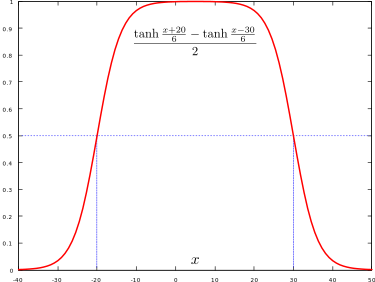
\includegraphics[width=2.5truein]{tiltshift-function.svg}
\caption{Exemplo de função de ponderação para tiltshift}

\end{figure}

Assumindo que \alpha(x) pondere a imagem original (denotada por
stem f(x,y)) e 1-\alpha(x) pondere a imagem borrada
(denotada por bf(x,y)), a composição g(x,y) = \alpha(x)
f(x,y) + (1-\alpha(x)) bf(x,y) produzirá o efeito de \texttt{tiltshift}
desejado.


O processo de ponderação pode ser realizado por intermédio da função
\texttt{multiply()} do OpenCV, destinada à multiplicação de matrizes
elemento-a-elemento. Cria-se a imagem que irá ponderar as linhas da
imagem original e seu negativo irá ponderar as linhas da imagem
borrada. A combinação linear dessas duas imagens fara o efeito
simulado de \texttt{tiltshift}. A Figura \hyperlink{fig-tiltshiftfunctionpondera}{Imagens para multiplicação} ilustra
possíveis imagens que poderiam ser usadas para ponderação no
processo. A da esquerda ponderaria a imagem original e a da direita a
imagem borrada.


\begin{figure}[h]{}
\centering
\includegraphics[width=2.5truein]{tiltshift-weight.jpg}
\caption{Exemplo de imagens geradas para ponderação no `tiltshift`}

\end{figure}

\hypertarget{x-exercícios}{\section{Exercícios}}
\begin{itemize}

\item Utilizando o programa \href{exemplos/addweighted.cpp}{exemplos/addweighted.cpp} como referência,
implemente um programa \texttt{tiltshift.cpp}. Três ajustes deverão ser
providos na tela da interface:

\begin{itemize}

\item um ajuste para regular a altura da região central que entrará em foco;

\item um ajuste para regular a força de decaimento da região borrada;

\item um ajuste para regular a posição vertical do centro da região que
 entrará em foco.
Finalizado o programa, a imagem produzida deverá ser salva em
 arquivo.

\end{itemize}

\item Utilizando o programa \href{exemplos/addweighted.cpp}{exemplos/addweighted.cpp} como referência,
implemente um programa \texttt{tiltshiftvideo.cpp}. Tal programa deverá ser
capaz de processar um arquivo de vídeo, produzir o efeito de
tilt-shift nos quadros presentes e escrever o resultado em outro
arquivo de vídeo. A ideia é criar um efeito de miniaturização de
cenas. Descarte quadros em uma taxa que julgar conveniente para
evidenciar o efeito de
\href{https://pt.wikipedia.org/wiki/Stop_motion}{stop motion}, comum
em vídeos desse tipo.

\end{itemize}


\hypertarget{x-filtragem-no-domínio-da-frequência}{\chapter{Filtragem no domínio da frequência}}
O objetivo desse capítulo é entender como se dá o uso da filtragem no
domínio da frequência usando a Transformada Discreta de Fourier
bidimensional.


A Transformada de Fourier é uma transformada capaz de expressar um
sinal contínuo como uma combinação de funções de base senoidais
ponderadas por coeficientes. A Transformada Discreta de Fourier, por
sua vez, é aplicada a sinais discretos, tais como imagens digitais.


Para uma imagem digital, a Transformada Discreta de Fourier (ou DFT),
é capaz de fornecer uma representação alternativa dessa imagem,
evidenciando degradações que não são facilmente tratadas no domínio
espacial. Exemplos de problemas dessa natureza são as interferências
senoidais nas transmissões de sinais analógicos ou padrões moiré
presentes em figuras antigas ou fotos de jornais. Um exemplo de
fotografia corrompida por um padrão moiré é mostrada na Figura
\hyperlink{fig-moire}{Interferências senoidais}. Note uma espécie de grade de pontos presentes nessa
imagem.


\begin{figure}[h]{}
\centering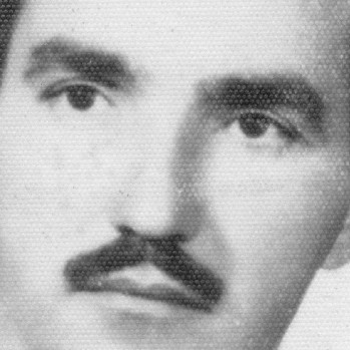
\includegraphics[width=2.5truein]{moire.png}
\caption{Exemplo de imagem corrompida por um padrão moiré}

\end{figure}

\begin{figure}[h]{}
\centering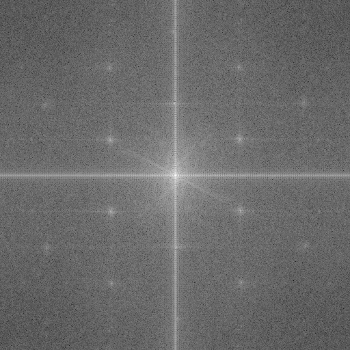
\includegraphics[width=2.5truein]{dftmoire.png}
\caption{Transformada Discreta de Fourier da imagem da Figura <<fig_moire>>}

\end{figure}

A Transformada Discreta de Fourier da imagem na Figura
\hyperlink{fig-dftmoire}{Interferências senoidais} é mostrada na Figura \hyperlink{fig-dftmoire}{Interferências senoidais}. Perceba um
conjunto de impulsos simétricos que surgem longe dos eixos,
destacando-se do restante do sinal transformado. São essas
contribuições as causadoras da grade de pontos.


Estabelecendo filtros especiais, é possível remover essas
contribuições da imagem transformada e, realizando a transformação
inversa, obter uma versão filtrada da imagem original.


A filtragem no domínio da Transformada de Fourier pode ser usada de
diversas formas. Nesta lição, mostra-se como criar um filtro ideal
passa baixas que remove as componentes de alta frequência de uma
sequência de vídeo. Nota-se que a imagem resultante do processo de
filtragem é borrada, dada a preservação apenas das componentes de
baixa frequência. Além disso, o exemplo simula uma interferência
senoidal (ruído coerente) adicionando à imagem transformada impulsos
simétricos na região de altas frequências.


Duas características de manipulação de imagens no domínio da
frequência são trabalhadas então: o projeto e uso de filtros
frequenciais e a manipulação direta do sinal transformado.


Para ilustrar o uso da Transformada Discreta de Fourier, considere o
exemplo mostrado na Listagem \hyperlink{exa-dft}{DFT}


\begin{verbatim}
#include <iostream>
#include <opencv2/opencv.hpp>
#include <opencv2/imgproc/imgproc.hpp>

#define RADIUS 20

using namespace cv;
using namespace std;

// troca os quadrantes da imagem da DFT
void deslocaDFT(Mat& image ){
  Mat tmp, A, B, C, D;

  // se a imagem tiver tamanho impar, recorta a regiao para
  // evitar cópias de tamanho desigual
  image = image(Rect(0, 0, image.cols & -2, image.rows & -2));
  int cx = image.cols/2;
  int cy = image.rows/2;

  // reorganiza os quadrantes da transformada
  // A B   ->  D C
  // C D       B A
  A = image(Rect(0, 0, cx, cy));
  B = image(Rect(cx, 0, cx, cy));
  C = image(Rect(0, cy, cx, cy));
  D = image(Rect(cx, cy, cx, cy));

  // A <-> D
  A.copyTo(tmp);  D.copyTo(A);  tmp.copyTo(D);

  // C <-> B
  C.copyTo(tmp);  B.copyTo(C);  tmp.copyTo(B);
}

int main(int , char**){
  VideoCapture cap;
  Mat imaginaryInput, complexImage, multsp;
  Mat padded, filter, mag;
  Mat image, imagegray, tmp;
  Mat_<float> realInput, zeros;
  vector<Mat> planos;

  // habilita/desabilita ruido
  int noise=0;
  // frequencia do ruido
  int freq=10;
  // ganho inicial do ruido
  float gain=1;

  // valor do ruido
  float mean;

  // guarda tecla capturada
  char key;

  // valores ideais dos tamanhos da imagem
  // para calculo da DFT
  int dft_M, dft_N;

  // abre a câmera default
  cap.open(0);
  if(!cap.isOpened())
    return -1;

  // captura uma imagem para recuperar as
  // informacoes de gravação
  cap >> image;

  // identifica os tamanhos otimos para
  // calculo do FFT
  dft_M = getOptimalDFTSize(image.rows);
  dft_N = getOptimalDFTSize(image.cols);

  // realiza o padding da imagem
  copyMakeBorder(image, padded, 0,
                 dft_M - image.rows, 0,
                 dft_N - image.cols,
                 BORDER_CONSTANT, Scalar::all(0));

  // parte imaginaria da matriz complexa (preenchida com zeros)
  zeros = Mat_<float>::zeros(padded.size());

  // prepara a matriz complexa para ser preenchida
  complexImage = Mat(padded.size(), CV_32FC2, Scalar(0));

  // a função de transferência (filtro frequencial) deve ter o
  // mesmo tamanho e tipo da matriz complexa
  filter = complexImage.clone();

  // cria uma matriz temporária para criar as componentes real
  // e imaginaria do filtro ideal
  tmp = Mat(dft_M, dft_N, CV_32F);

  // prepara o filtro passa-baixas ideal
  for(int i=0; i<dft_M; i++){
    for(int j=0; j<dft_N; j++){
      if((i-dft_M/2)*(i-dft_M/2)+(j-dft_N/2)*(j-dft_N/2) < RADIUS*RADIUS){
        tmp.at<float> (i,j) = 1.0;
      }
    }
  }

  // cria a matriz com as componentes do filtro e junta
  // ambas em uma matriz multicanal complexa
  Mat comps[]= {tmp, tmp};
  merge(comps, 2, filter);

  for(;;){
    cap >> image;
    cvtColor(image, imagegray, CV_BGR2GRAY);
    imshow("original", imagegray);

    // realiza o padding da imagem
    copyMakeBorder(imagegray, padded, 0,
                   dft_M - image.rows, 0,
                   dft_N - image.cols,
                   BORDER_CONSTANT, Scalar::all(0));

    // limpa o array de matrizes que vao compor a
    // imagem complexa
    planos.clear();
    // cria a compoente real
    realInput = Mat_<float>(padded);
    // insere as duas componentes no array de matrizes
    planos.push_back(realInput);
    planos.push_back(zeros);

    // combina o array de matrizes em uma unica
    // componente complexa
    merge(planos, complexImage);

    // calcula o dft
    dft(complexImage, complexImage);

    // realiza a troca de quadrantes
    deslocaDFT(complexImage);

    // aplica o filtro frequencial
    mulSpectrums(complexImage,filter,complexImage,0);

    // limpa o array de planos
    planos.clear();
    // separa as partes real e imaginaria para modifica-las
    split(complexImage, planos);

    // usa o valor medio do espectro para dosar o ruido
    mean = abs(planos[0].at<float> (dft_M/2,dft_N/2));

    // insere ruido coerente, se habilitado
    if(noise){
      // F(u,v) recebe ganho proporcional a F(0,0)
      planos[0].at<float>(dft_M/2 +freq, dft_N/2 +freq) +=
        gain*mean;

      planos[1].at<float>(dft_M/2 +freq, dft_N/2 +freq) +=
        gain*mean;

      // F*(-u,-v) = F(u,v)
      planos[0].at<float>(dft_M/2 -freq, dft_N/2 -freq) =
        planos[0].at<float>(dft_M/2 +freq, dft_N/2 +freq);

      planos[1].at<float>(dft_M/2 -freq, dft_N/2 -freq) =
        -planos[1].at<float>(dft_M/2 +freq, dft_N/2 +freq);

    }

    // recompoe os planos em uma unica matriz complexa
    merge(planos, complexImage);

    // troca novamente os quadrantes
    deslocaDFT(complexImage);

	cout << complexImage.size().height << endl;
    // calcula a DFT inversa
    idft(complexImage, complexImage);

    // limpa o array de planos
    planos.clear();

    // separa as partes real e imaginaria da
    // imagem filtrada
    split(complexImage, planos);

    // normaliza a parte real para exibicao
    normalize(planos[0], planos[0], 0, 1, CV_MINMAX);
    imshow("filtrada", planos[0]);

    key = (char) waitKey(10);
    if( key == 27 ) break; // esc pressed!
    switch(key){
      // aumenta a frequencia do ruido
    case 'q':
      freq=freq+1;
      if(freq > dft_M/2-1)
        freq = dft_M/2-1;
      break;
      // diminui a frequencia do ruido
    case 'a':
      freq=freq-1;
      if(freq < 1)
        freq = 1;
      break;
      // amplifica o ruido
    case 'x':
      gain += 0.1;
      break;
      // atenua o ruido
    case 'z':
      gain -= 0.1;
      if(gain < 0)
        gain=0;
      break;
      // insere/remove ruido
    case 'e':
      noise=!noise;
      break;
    }
  }
  return 0;
}
\end{verbatim}

\hypertarget{x-descrição-do-programa-\texttt{dft.cpp}}{\section{Descrição do programa \texttt{dft.cpp}}}
O programa funciona capturando continuamente quadros da primeira
câmera disponível, calcula a Transformada de Fourier e realiza duas
operações:


\begin{itemize}

\item Filtragem no domínio da frequência usando filtro ideal passa-baixas
com frequência de corte de 20 pixels.

\item Inserção de ruído coerente com frequência ajustável pela variável
\emph{freq} , nas posições F(freq, freq) e F(-freq,-freq).

\end{itemize}


Para aplicar o filtro, é necessário que o sinal transformado seja
deslocado de modo que a origem do sinal fique posicionada no centro da
imagem, como ilustra a Figura \hyperlink{fig-dftshift}{Deslocamento da imagem transformada}.


\begin{figure}[h]{}
\centering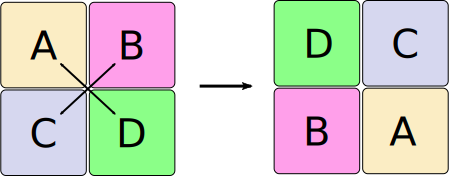
\includegraphics[width=2.5truein]{dftshift.svg}
\caption{Deslocamento da imagem transformada}

\end{figure}

A operação de deslocamento é realizada pela função \texttt{deslocaDft()}. Ela
recebe a referência para a matriz que contém a imagem transformada e
troca seus quadrantes. Caso a imagem possua tamanho \textbf{ímpar}, ela é
diminuída de tamanho em \textbf{um pixel} para que a troca dos quadrantes
seja feita usando tamanhos imagens de iguais. Normalmente, trata-se a
imagem que será submetida ao cálculo da DFT para que possua dimensões
de ordem par, de sorte que essa linha não deverá alterar o tamanho das
imagens usualmente fornecidas.


\begin{verbatim}
// habilita/desabilita ruido
int noise=0;
// frequencia do ruido
int freq=10;
// ganho inicial do ruido
float gain=1;
\end{verbatim}

Essa são variáveis que regulam um ruído coerente que pode ser
adicionado ao sinal filtrado para simular uma inteferência. A variável
\texttt{noise} pode assumir os valores \texttt{0} ou \texttt{1}, indicando se a
inteferência será aplicada ou não, respectivamente. Essa variável é
alterada de \texttt{0->1} ou \texttt{1->0} quando a tecla  é pressionada.


As variáveis \texttt{freq} e \texttt{gain} regulam a frequência do ruído coerente e
sua intensidade. Esta última é adicionada à imagem transformada como
uma proporção ao valor de F(0,0), valor médio dos tons de cinza
da imagem capturada. Escolheu-se o valor de F(0,0) para que a
ponderação da inteferência ficasse atrelada a cada imagem, causando um
efeito visual mais convincente.


\begin{verbatim}
dft_M = getOptimalDFTSize(image.rows);
dft_N = getOptimalDFTSize(image.cols);
\end{verbatim}

A função \texttt{getOptimalDFTSize()} identifica os melhores valores com base
no tamanho fornecido para acelerar o processo de cálculo da DFT com
base em algum algoritmo otimizado. Segundo a documentação do OpenCV,
valores múltiplos de dois, três e cinco produzem resultados
melhores. Os valores de tamanho ideal para a quantidade de linhas e
colunas da imagem são armazenados nas variáveis \texttt{dft_M} e \texttt{dft_N},
respectivamente.


\begin{verbatim}
copyMakeBorder(image, padded, 0,
               dft_M - image.rows, 0,
               dft_N - image.cols,
               BORDER_CONSTANT, Scalar::all(0));
\end{verbatim}

A função \texttt{copyMakeBorder()} cria uma versão da imagem fornecida com
uma borda preenchida com \emph{zeros} e ajustada ao tamanho ótimo para
cálculo da DFT, conforme indicado pelo uso da função
\texttt{getOptimalDFTSize()}. Para uma imagem \texttt{image} fornecida, a saída é
produzida na imagem \texttt{padded}. Perceba que, caso a imagem fornecida já
possua dimensões apropriadas, a imagem de saída será igual à de
entrada.


\begin{verbatim}
// parte imaginaria da matriz complexa (preenchida com zeros)
zeros = Mat_<float>::zeros(padded.size());

// prepara a matriz complexa para ser preenchida
complexImage = Mat(padded.size(), CV_32FC2, Scalar(0));
\end{verbatim}

Esse trecho de código constrói a matriz uma matriz de zeros tipo float
e uma matriz complexa que serão necessárias para o cálculo da DFT. A
matriz de zeros é usada para compor, juntamente com a imagem
capturada, a componente complexa que será fornecida à função que
calcula a Tranformada de Fourier.


\begin{verbatim}
// a função de transferência (filtro frequencial) deve ter o
// mesmo tamanho e tipo da matriz complexa
filter = complexImage.clone();

// cria uma matriz temporária para criar as componentes real
// e imaginaria do filtro ideal
tmp = Mat(dft_M, dft_N, CV_32F);

// prepara o filtro passa-baixas ideal
for(int i=0; i<dft_M; i++){
 for(int j=0; j<dft_N; j++){
    if((i-dft_M/2)*(i-dft_M/2)+(j-dft_N/2)*(j-dft_N/2) < RADIUS*RADIUS){
      tmp.at<float> (i,j) = 1.0;
    }
  }
}

// cria a matriz com as componentes do filtro e junta
// ambas em uma matriz multicanal complexa
Mat comps[]= {tmp, tmp};
merge(comps, 2, filter);
\end{verbatim}

O filtro ideal passa baixas é preparado com base na matriz complexa
\texttt{complexImage} previamente montada. Esse filtro, armazenado na matriz
\texttt{filter} \textbf{DEVE SER DO MESMO TAMANHO E TIPO DA IMAGEM COMPLEXA} para
que a função de filtragem funcione corretamente. O filtro ideal é
criado desenhando-se no centro da imagem complexa um círculo de raio
igual a \texttt{RADIUS} com todos os valores preenchidos com \texttt{1}. Fora desse
raio, o valor do filtro é igual a \texttt{0}.


Como as duas componentes da imagem do filtro - real e complexa -
precisam ter exatamente os mesmos valores, uma matriz temporária \texttt{tmp}
armazena os valores do filtro, que em seguida são combinadas com a
função \texttt{merge()} para montar a matriz do filtro.


\begin{verbatim}
// limpa o array de matrizes que vao compor a
// imagem complexa
planos.clear();
// cria a compoente real
realInput = Mat_<float>(padded);
// insere as duas componentes no array de matrizes
planos.push_back(realInput);
planos.push_back(zeros);
// combina o array de matrizes em uma unica
// componente complexa
merge(planos, complexImage);
\end{verbatim}

Em cada passada no \emph{loop} infinito do programa, uma imagem capturada
da câmera é redimensionada (quando necessário) e preparada para o
cálculo da DFT.


Um vetor auxiliar \texttt{planos} é usado para montar a matriz
complexa. Inicialmente, o vetor é limpo para armazenar as novas
contribuições. Cria-se uma matriz \texttt{realInput} do tipo \texttt{float}, com
base na imagem resultante da operação de \emph{padding}. Tanto essa quanto
a matriz de zeros são inseridas no array de planos. O array é, então,
combinado usando a função \texttt{merge()} para montar a matriz complexa.


\begin{verbatim}
// calcula o dft
dft(complexImage, complexImage);

// realiza a troca de quadrantes
deslocaDFT(complexImage);
\end{verbatim}

O cálculo do DFT é realizado. Perceba que tanto a matriz de entrada
quanto a de saída passadas como parâmetro podem ser a
mesma. Finalizado o cálculo da DFT, a função \texttt{deslocaDFT()} realiza a
troca de quadrantes.


\begin{verbatim}
// aplica o filtro frequencial
mulSpectrums(complexImage,filter,complexImage,0);
\end{verbatim}

Agora, o processo de filtragem no domínio da frequência é propriamente
realizado. A função \texttt{mulSpectrums()} recebe pelo menos quatro
argumentos: a imagem a ser filtrada, o filtro, a imagem onde deverá
ser lançada a saída (que pode ser a mesma matriz de entrada), e flags
de operação. Normalmente, esse flag não é usado, adicionando-se
simplesmente \texttt{0} ao seu valor.


\begin{verbatim}
// limpa o array de planos
planos.clear();
// separa as partes real e imaginaria para modifica-las
split(complexImage, planos);

// usa o valor medio do espectro para dosar o ruido
mean = abs(planos[0].at<float> (dft_M/2,dft_N/2));
// insere ruido coerente, se habilitado
if(noise){
  // F(u,v) recebe ganho proporcional a F(0,0)
  planos[0].at<float>(dft_M/2 +freq, dft_N/2 +freq) +=
   gain*mean;

  planos[1].at<float>(dft_M/2 +freq, dft_N/2 +freq) +=
    gain*mean;

  // F*(-u,-v) = F(u,v)
  planos[0].at<float>(dft_M/2 -freq, dft_N/2 -freq) =
    planos[0].at<float>(dft_M/2 +freq, dft_N/2 +freq);

  planos[1].at<float>(dft_M/2 -freq, dft_N/2 -freq) =
    -planos[1].at<float>(dft_M/2 +freq, dft_N/2 +freq);
}
\end{verbatim}

Esse trecho realiza a simulação da inteferência por ruído
coerente. Inicialmente, o array de planos é limpo para receber as
partes real e imaginária da imagem filtrada. Ele é preenchido pela
função \texttt{split()} que realiza a divisão da imagem complexa em dois
arrays reais. Estes arrays ficam contidos em \texttt{planos[0]} (componente
real) e \texttt{planos[1]} (componente imaginária).


O trecho seguinte introduz o ruído nas posições da imagem localicadas
em F(freq, freq) e F(-freq,-freq). Veja que
nas equações é dado um deslocamento adicional nos índices dos arrays
igual a \texttt{(dft_M/2, dft_N/2)}, já que a origem da Transformada de Fourier
está posicionada no centro da imagem. Observe também que as
ponderações são realizadas utilizando as propriedades de simetria.


\begin{verbatim}
// recompoe os planos em uma unica matriz complexa
merge(planos, complexImage);

// troca novamente os quadrantes
deslocaDFT(complexImage);

// calcula a DFT inversa
idft(complexImage, complexImage);
\end{verbatim}

Uma vez inserida a interferência, os planos reais são novamente
fundidos em uma matriz complexa. Essa matriz deve ter seus quadrantes
trocados para que seja realizado cálculo da Transformada de Fourier
inversa usando a função \texttt{idft()}.


\begin{verbatim}
// limpa o array de planos
planos.clear();

// separa as partes real e imaginaria da
// imagem filtrada
split(complexImage, planos);

// normaliza a parte real para exibicao
normalize(planos[0], planos[0], 0, 1, CV_MINMAX);
imshow("filtrada", planos[0]);
\end{verbatim}

A imagem complexa é separada em suas componentes real e imaginária nos
elementos do array \texttt{planos}. A matriz \texttt{planos[0]} conterá a imagem
processada. Ela tem seus valores normalizados na faixa [0,1]
para exibição na tela.


A sequência do programa apenas trata opções de menu que realizam
modificações no ganho e na frequência de corte da interferência
simulada. As opções do menu são descritas na tabela seguinte:


\begin{center}
\begin{tabular}{|c|c|}
\hline
 & aumenta a frequência da interferência \\ 
 & diminui a frequência da interferência \\ 
 & aumenta o ganho da inteferência \\ 
 & diminui o ganho da interferência \\ 
 & habilita/desabilita o efeito da interferência \\ 
\hline
\end{tabular}
\end{center}

\hypertarget{x-exercícios}{\section{Exercícios}}
\begin{itemize}

\item Utilizando o programa \href{exemplos/dft.cpp}{exemplos/dft.cpp} como referência,
implemente o filtro homomórfico para melhorar imagens com iluminação
irregular. Crie uma cena mal iluminada e ajuste os parâmetros do
filtro homomórfico para corrigir a iluminação da melhor forma
possível. Assuma que a imagem fornecida é em tons de cinza.

\end{itemize}


\hypertarget{x-detecção-de-bordas-com-o-algoritmo-de-canny}{\chapter{Detecção de bordas com o algoritmo de Canny}}
O detector de bordas de Canny é sabidamente reconhecido como um dos
mais rápidos e eficientes algoritmos para encontrar descontinuidades
em uma imagem. Ele produz como resultado uma imagem binária contendo
os pontos de borda obtidos a partir de uma imagem, para um conjunto de
parâmetros de configuração.


Em linhas gerais, o algoritmo de Canny procura descobrir bordas situadas
em máximos locais do gradiente de uma image, e pode ser sumarizado
pelos seguintes passos:


\begin{enumerate}

\item{Convolução com o filtro Gaussiano, cálculo da magnitude e ângulo do
gradiente.}

\item{Afinação das cristas largas do gradiente.}

\begin{enumerate}

\item{Classificação dos pontos quanto às orientações Horizontal,
Vertical, +45^\text{o}, e -45^\text{o}
(intervalos de \pm 22.5^\text{o}).}

\item{Para os vizinhos na orientação determinada para o pixel, verificar
os seus gradientes.}

\item{Supressão de não máximos: se o valor da magnitude do gradiente
M(x,y) for inferior a pelo menos um de seus vizinhos, faça
g_N(x,y)=0; caso contrário, faça g_N(x,y) =
M(x,y). A imagem g_N(x,y) é a imagem com supressão.}

\end{enumerate}

\item{Limiarização com histerese é usada para a quebra do contorno (borda
tracejada).}

\begin{enumerate}

\item{Dois limiares T_1 e T_2. T_1 > T_2 são usados.}

\item{Se o pixel é tal que g_N(x,y) \ge T_1, é assumido como ponto de borda forte.}

\item{Para os pixels restantes, aqueles em que g_N(x,y) \ge T_2, são assumidos como ponto de borda fraco.}

\item{Para todos os vizinhos dos pontos de borda fraco, procurar nos seus
8-vizinhos se há algum ponto de borda forte. Caso haja, este é marcado
como parte da fronteira.}

\item{Sugestão de Canny: T_H/T_L = 3/1, ou T_H/T_L =2/1}

\end{enumerate}

\end{enumerate}


Um exemplo de aplicação desse algoritmo na imagem da Figura
\hyperlink{fig-canny-exemplo}{Exemplo para o detector de Canny} é mostrado na Figura \hyperlink{fig-canny}{Detecção de bordas usando o filtro de Canny}. Observe que
as bordas encontradas são bem localizadas e geralmente possuem
espessura igual a 1.


\begin{figure}[h]{}
\centering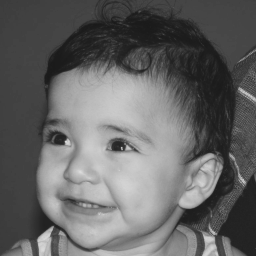
\includegraphics[width=2.5truein]{biel.png}
\caption{Exemplo para o detector de Canny}

\end{figure}

\begin{figure}[h]{}
\centering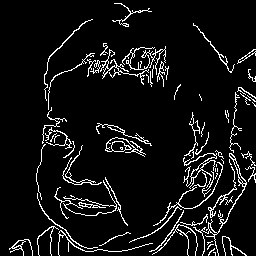
\includegraphics[width=2.5truein]{canny.png}
\caption{Detecção de bordas usando o filtro de Canny}

\end{figure}

O programa que gerou essa imagem é mostrado no Exemplo \hyperlink{exa-canny}{Canny}.


\begin{verbatim}
#include <iostream>
#include "opencv2/opencv.hpp"

using namespace std;
using namespace cv;

int top_slider = 10;
int top_slider_max = 200;

char TrackbarName[50];

Mat image, border;

void on_trackbar_canny(int, void*){
  Canny(image, border, top_slider, 3*top_slider);
  imshow("canny", border);
}

int main(int argc, char**argv){
  int width, height;

  image= imread(argv[1],CV_LOAD_IMAGE_GRAYSCALE);

  width=image.size().width;
  height=image.size().height;

  sprintf( TrackbarName, "Threshold inferior", top_slider_max );

  namedWindow("canny",1);
  createTrackbar( TrackbarName, "canny",
                &top_slider,
                top_slider_max,
                on_trackbar_canny );

  on_trackbar_canny(top_slider, 0 );

  waitKey();
  imwrite("cannyborders.png", border);
  return 0;
}
\end{verbatim}

Para compilar e executar o programa
\href{exemplos/canny.cpp}{canny.cpp}, salve-o juntamente com os arquivo
\href{exemplos/Makefile}{Makefile} e a imagem
\href{figs/biel.png}{biel.png} em um diretório e execute a seguinte
seqüência de comandos:


\begin{verbatim}
$ make canny
$ ./canny biel.png
\end{verbatim}

O programa disponibilizará uma \emph{scrollbar} que regula o valor do
limiar T_1. O valor do limiar T_2 é
determinado automaticamente usando a proporção T_1 = 3
T_1. Ao ser finalizado - quando uma tecla é pressionada - o programa
escreve a imagem de bordas no arquivo de nome \texttt{cannyborders.png}.


Valores diferentes para o limiar escolhido produzem imagens de bordas
diferentes.


A função de destaque nesse programa exemplo é apenas a função
\texttt{Canny()}.


\begin{verbatim}
Canny(image, border, top_slider, 3*top_slider);
\end{verbatim}

Os dois primeiros argumentos indicam a imagem a ser processada, a
matriz onde a imagem de bordas será escrita, e os limiares
T_1 e T_2, neste caso representado pelas
quantidades  \texttt{top_slider} e \texttt{3*top_slider}.


\hypertarget{x-canny-e-a-arte-com-pontilhismo}{\chapter{Canny e a arte com pontilhismo}}
O algoritmo de Canny de fato é útil para diversas aplicações em
processamento de imagens e visão artificial. Informações de bordas
podem ser usadas para melhorar algoritmos de segmentação automática ou
para encontrar objetos em cenas e pontos de interesse.


Entretanto, nesta lição, a proposta de uso do algoritmo é para
desenvolver arte digital. A ideia é usar uma imagem de referência para
criar uma nova imagem usando efeitos artísticos pontilhistas.


O pontilhismo é uma técnica de desenho impressionista onde o quadro é
pintado usando apenas pontos. Um dos artistas pioneiros nessa técnica
foi \href{https://en.wikipedia.org/wiki/Georges_Seurat}{George
Seurat}. Vários dos seus trabalhos podem ser vistos \emph{online} no site
\href{http://www.georgesseurat.org/}{georgesseurat.org}.


Simular no computador um efeito pontilhista não é muito
trabalhoso. Uma estratégia simples é utilizar uma imagem de referência
e criar uma outra imagem desenhada usando pequenos círculos. Em suma,
percorre-se a imagem de referência e para cada pixel, desenha-se um
círculo com a mesma cor na posição correspondente na imagem
pontilhista.


Efeitos pontilhistas interessantes podem ser criados com variantes
simples dessa técnica. Exemplo: pular sequências de pixels na imagem
de referência para dar a impressão de que os pontos estão separados na
tela - isso é bastante comum na arte pontilhista. Outro efeito
interessante é realizar deslocamentos aleatórios nos centros dos
círculos, para que a imagem gerada permaneca menos
artificial. Finalmente, é razoável percorrer a matriz de referência
usando uma sequência aleatória, principalmente quando a técnica
pontilhista realiza a sobreposição de círculos.


Um exemplo de imagem pontilhista é mostrada na Figura \hyperlink{fig-pontilhismo}{Pontilhismo}.


\begin{figure}[h]{}
\centering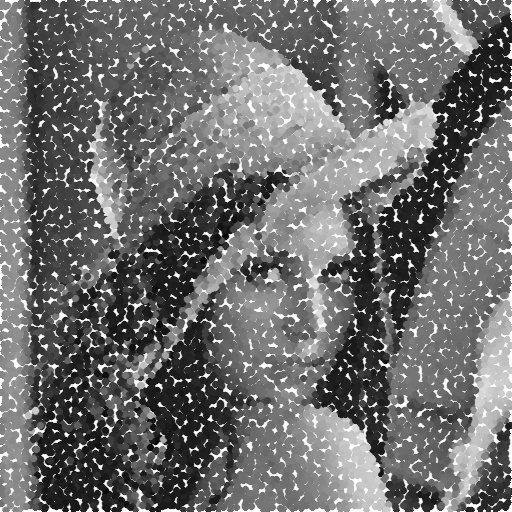
\includegraphics[width=2.5truein]{pontos.png}
\caption{Imagem pontilhista}

\end{figure}

O programa que gerou essa imagem é mostrado no Exemplo \hyperlink{exa-pontilhismo}{Pontilhismo}.


\begin{verbatim}
#include <iostream>
#include <opencv2/opencv.hpp>
#include <fstream>
#include <iomanip>
#include <vector>
#include <algorithm>
#include <numeric>
#include <ctime>
#include <cstdlib>

using namespace std;
using namespace cv;

#define STEP 5
#define JITTER 3
#define RAIO 3

int main(int argc, char** argv){
  vector<int> yrange;
  vector<int> xrange;

  Mat image, frame, points;

  int width, height, gray;
  int x, y;

  image= imread(argv[1],CV_LOAD_IMAGE_GRAYSCALE);

  srand(time(0));

  if(!image.data){
	cout << "nao abriu" << argv[1] << endl;
    cout << argv[0] << " imagem.jpg";
    exit(0);
  }

  width=image.size().width;
  height=image.size().height;

  xrange.resize(height/STEP);
  yrange.resize(width/STEP);

  iota(xrange.begin(), xrange.end(), 0);
  iota(yrange.begin(), yrange.end(), 0);

  for(uint i=0; i<xrange.size(); i++){
    xrange[i]= xrange[i]*STEP+STEP/2;
  }

  for(uint i=0; i<yrange.size(); i++){
    yrange[i]= yrange[i]*STEP+STEP/2;
  }

  points = Mat(height, width, CV_8U, Scalar(255));

  random_shuffle(xrange.begin(), xrange.end());

  for(auto i : xrange){
    random_shuffle(yrange.begin(), yrange.end());
    for(auto j : yrange){
      x = i+rand()%(2*JITTER)-JITTER+1;
      y = j+rand()%(2*JITTER)-JITTER+1;
      gray = image.at<uchar>(x,y);
      circle(points,
             cv::Point(y,x),
             RAIO,
             CV_RGB(gray,gray,gray),
             -1,
             CV_AA);
    }
  }
  imwrite("pontos.jpg", points);
  return 0;
}
\end{verbatim}

Para compilar e executar o programa
\href{exemplos/pontilhismo.cpp}{pontilhismo.cpp}, salve-o juntamente com
o arquivo \href{exemplos/Makefile}{Makefile} e a imagem
\href{figs/biel.png}{biel.png} em um diretório e execute a seguinte
seqüência de comandos:


\begin{verbatim}
$ make pontilhismo
$ ./pontilhismo biel.png
\end{verbatim}

\hypertarget{x-descrição-do-programa-\texttt{pontilhismo.cpp}}{\chapter{Descrição do programa \texttt{pontilhismo.cpp}}}
O programa \texttt{pontilhismo.cpp} não introduz novas funcionalidades da
biblioteca de programação OpenCV. Entretanto, algumas classes da
\href{http://www.cplusplus.com/reference/stl/}{STL}, a biblioteca padrão
de gabaritos do C++ estão presentes no código para facilitar a criação
de alguns efeitos. Logo, é conveniente discorrer um pouco sobre seu
uso no exemplo.


\begin{verbatim}
vector<int> yrange;
vector<int> xrange;
\end{verbatim}

Define-se dois arrays de índices que servirão para identificar
elementos da imagem de referência. Os tamanhos dos arrays \texttt{xrange} e
\texttt{yrange} são determinados como frações da altura e da largura da
imagem, respectivamente. Isso é feito para que na geração da imagem
pontilhista, apenas alguns pontos sejam amostrados na imagem de
referência, evitando sobrecarga visual.


A grandeza \texttt{STEP} define o passo usado para varrer a imagem de
referência. No exemplo, usamos \texttt{STEP} igual a 5 pixels, ou seja,
considerando as duas dimensões da imagem, apenas 1 em cada
5 \times 5 = 25 pixels de uma janela é usado para criar um
círculo.


\begin{verbatim}
iota(xrange.begin(), xrange.end(), 0);
iota(yrange.begin(), yrange.end(), 0);

for(uint i=0; i<xrange.size(); i++){
  xrange[i]= xrange[i]*STEP+STEP/2;
}

for(uint i=0; i<yrange.size(); i++){
  yrange[i]= yrange[i]*STEP+STEP/2;
}
\end{verbatim}

Os arrays \texttt{xrange} e \texttt{yrange} são preenchidos com valores sequenciais
iniciando em \texttt{0} e, em seguida, esses valores recebem um ganho igual a
\texttt{STEP} e um deslocamento \texttt{STEP/2}, para que o processo de amostragem
na imagem de referência se dê no centro da janela.


\begin{verbatim}
random_shuffle(xrange.begin(), xrange.end());
\end{verbatim}

A função \texttt{random_shuffle()} recebe como parâmetros 2 iteradores: uma
para o início do array e outro para o final. Como resultado, a função
embaralha aleatoriamente todos seus elementos. Se observado, esse
processo é feito uma vez para o array de índices das linhas -
\texttt{xrange} - e, para cada linha, embaralha-se o array de índices das
colunas - \texttt{yrange}.


Os loops descritos por \texttt{for(auto i : xrange)} e \texttt{for(auto j : yrange)}
são construções na especificação \texttt{C++11} e servem para fazer as
variáveis \texttt{i} e \texttt{j} assumirem, a cada passada no loop, os valores dos
arrays \texttt{xrange} e \texttt{yrange} de forma consecutiva.


\begin{verbatim}
x = i+rand()%(2*JITTER)-JITTER+1;
y = j+rand()%(2*JITTER)-JITTER+1;
\end{verbatim}

O valor das coordenadas do ponto cujo tom de cinza será amostrado na
imagem de referência é determinado pela posição do centro da janela
mais um deslocamento aleatório em ambas as direções. Esse deslocamento
é determinado pela grandeza \texttt{JITTER} (igual a 3 pixels).


Variações das grandezas \texttt{STEP} e \texttt{JITTER} podem ser modificadas para
uso em imagens de tamanhos diferentes.


\begin{verbatim}
circle(points, cv::Point(y,x), RAIO, CV_RGB(gray,gray,gray), -1, CV_AA);
\end{verbatim}

A função \texttt{circle()} é usada para traçar um círculo de raio
especificado em um ponto determinado pelo usuário. O círculo é
desenhado usando preenchimento sólido e, dada a presença do parâmetro
\texttt{CV_AA}, este será desenhado usando técnicas de \emph{antialiasing}. Assim,
o círculo terá bordas não serrilhadas, produzindo um efeito visual
agradável na imagem pontilhista.


\hypertarget{x-exercícios}{\section{Exercícios}}
\begin{itemize}

\item Utilizando os programas \href{exemplos/canny.cpp}{exemplos/canny.cpp} e
\href{exemplos/pontilhismo.cpp}{exemplos/pontilhismo.cpp} como referência, implemente um
programa \texttt{cannypoints.cpp}. A idéia é usar as bordas produzidas pelo
algoritmo de Canny para melhorar a qualidade da imagem pontilhista
gerada. A forma como a informação de borda será usada é
livre. Entretanto, são apresentadas algumas sugestões de técnicas
que poderiam ser utilizadas:

\begin{itemize}

\item Desenhar pontos grandes na imagem pontilhista básica;

\item Usar a posição dos pixels de borda encontrados pelo algoritmo de
Canny para desenhar pontos nos respectivos locais na imagem gerada.

\item Experimente ir aumentando os limiares do algoritmo de Canny e, para
cada novo par de limiares, desenhar círculos cada vez menores nas
posições encontradas. A Figura \hyperlink{fig-lenapontilhista}{Pontilhismo aplicado à imagem Lena} foi
desenvolvida usando essa técnica.

\end{itemize}

\item Escolha uma imagem de seu gosto e aplique a técnica que você
desenvolveu.

\item Descreva no seu relatório detalhes do procedimento usado para criar
sua técnica pontilhista.

\end{itemize}


\begin{figure}[h]{}
\centering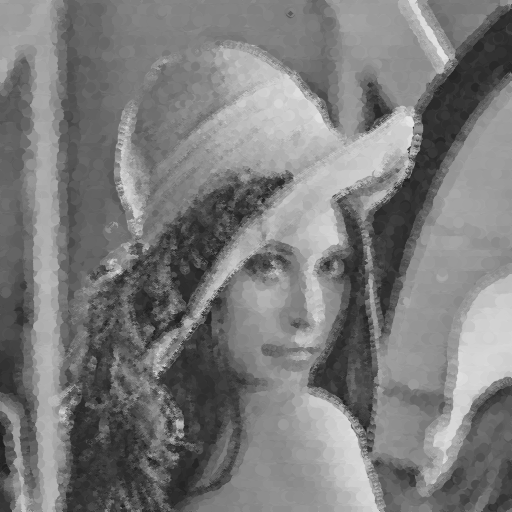
\includegraphics[width=2.5truein]{lenapontilhista.png}
\caption{Pontilhismo aplicado à imagem Lena}

\end{figure}

\end{document}

